\chapter{The acquisition of data}

\section{The LHC}
  The Large Hadron Collider (LHC) is a particle accelerator and collider which runs underground near Geneva, Switzerland. Figure \ref{fig:lhc_tunnel} shows the outline of the beam pipe under the greater Geneva area at the Swiss-French border. The beam pipe is 26.7 km long and is housed in a tunnel between 45 and 170 meters underground. This thesis is concerned with the proton-proton collisions at the LHC, which constitute the majority of the run-time. 

  The protons in these collisions are sourced from hydrogen gas, which has its electrons stripped at the CERN Meyran facility and are then sent through several smaller accelerators before being injected into the LHC at 450 GeV. The LHC then accelerates the protons such that they achieve a kinetic energy of 6.5 TeV in the lab frame, the collisions between the beams then have a center of mass energy, $\sqrt{s}$, of 13 TeV \cite{LHC_JINST}, \cite{LHC_TDR}. 

  Protons are injected into the LHC in bunches, each containing approximately $10^{12}$ protons \cite{Lumi_unc}, and are accelerated in both clockwise and counterclockwise directions in two separate high vacuum beam pipes. About these beam pipes, superconducting dipole magnets guide the beams around the circular path, and quadrupole and octopole magnets ensure the beams stay focused and collimated.

  The proton bunches extend approximately 55 mm in length and are spaced such that the time between bunch crossings at any particular point in the beam pipe is approximately 25 ns at full energy. The four points, 1, 2, 5, and 8, distinguished in figure \ref{fig:lhc_tunnel}, the beams are crossed and the protons are given a chance to collide. In an average head-on bunch crossing, approximately 20 proton-proton pairs will collide and create deposits of energy in the detectors wrapped around the interaction points. For the analysis presented in this thesis, data was collected during the 2016 LHC run, corresponding to a usable integrated luminosity of 35.9 fb$^{-1}$ collected by the CMS detector. Typical instantaneous luminosities during this time period were on the order of $10^{34}$ cm$^{-2}$ s$^{-1} = 10^7$ Hz fb$^{-1}$, as can be seen in figure \ref{fig:lumi_stats} \cite{lumi_twiki}.

  \begin{figure}[h!]
    \centering
    \includegraphics[width=.7\textwidth]{figures/lhc_underground.jpg}
    \caption{Outline of the LHC tunnel around the greater Geneva area. The accelerator is 26.7 km long and is housed in a tunnel between 45 and 170 meters underground. Taken from \cite{LHC_underground}}
    \label{fig:lhc_tunnel}
  \end{figure}

  \begin{figure}[h!]
    \centering
    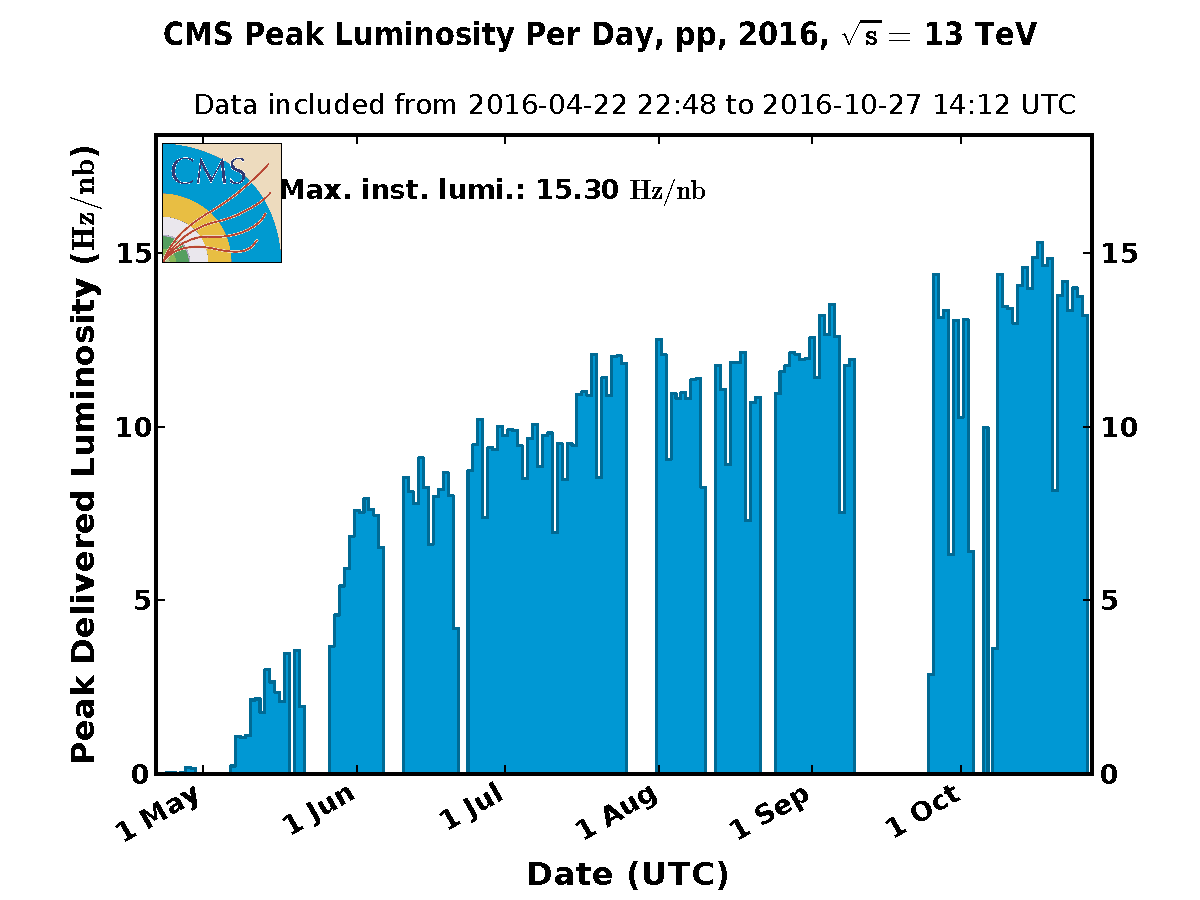
\includegraphics[width=.48\textwidth]{figures/peak_lumi_per_day_pp_2016.pdf}
    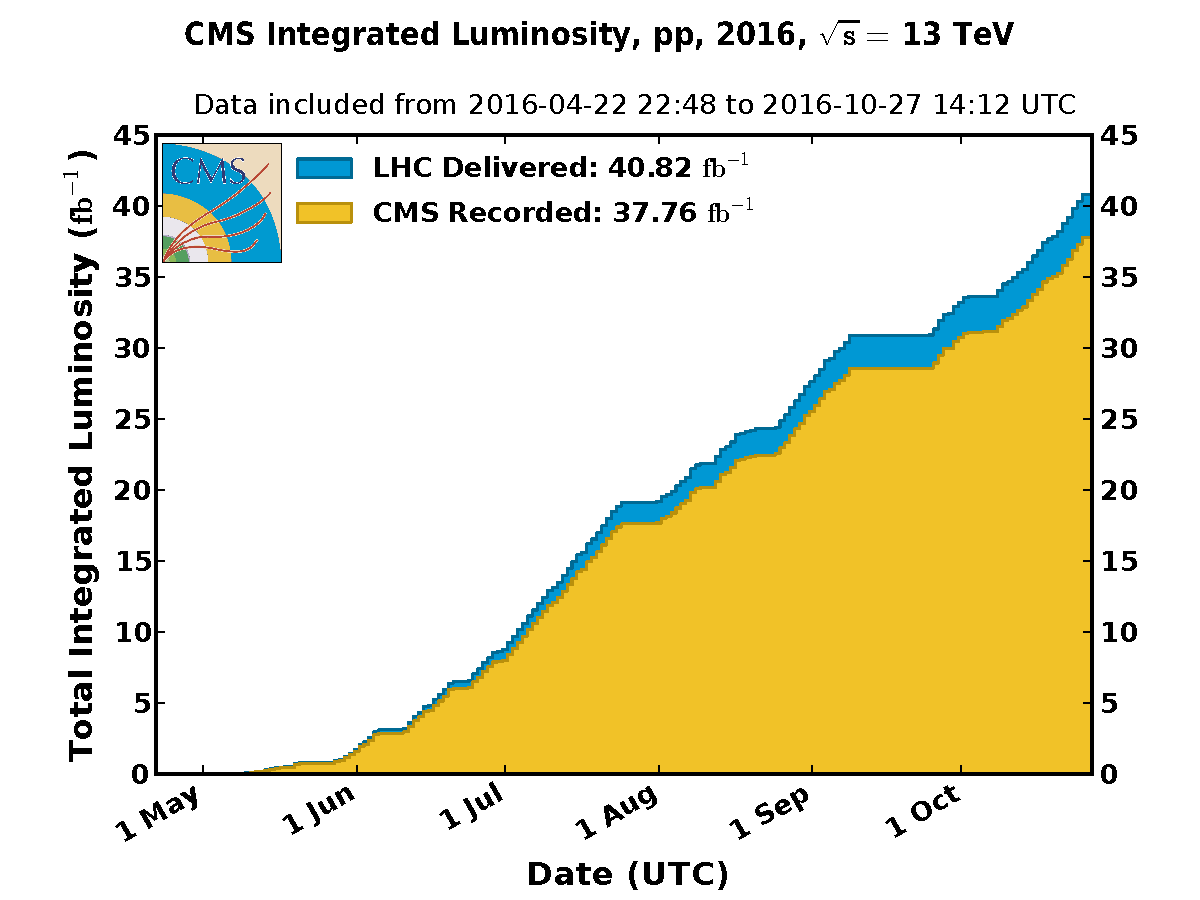
\includegraphics[width=.48\textwidth]{figures/int_lumi_per_day_cumulative_pp_2016.pdf}
    \caption{Peak instantaneous and integrated luminosity over time during the 2016 LHC proton-proton run delivered to the CMS detector. The difference between the 35.9 fb$^{-1}$ used in this analysis and the shown 37.76 fb$^{-1}$ comes from the omission of certain run periods where the detector was not operating optimally for the detection of leptons. Taken from \cite{lumi_twiki}.}
    \label{fig:lumi_stats}
  \end{figure}

  \subsection{What gets made?} \label{sec:what_gets_made}
    As mentioned in the previous section, the typical number of collisions leading to measurable energy deposits in the detector is 20 per bunch crossing. Figure \ref{fig:lhc_decay_modes} shows cross section for various proton-proton final states as a function of center of mass energy. Notice that the vast majority of the collisions result in low energy jet production or elastic scattering. 

    The analysis presented in this thesis is concerned with the production of Z bosons, whose production cross section is denoted as $\sigma_\text{Z}$ in the figure. Given the instantaneous luminosity of $10^{34}$ cm$^{-2}$ s$^{-1}$, the production cross section corresponds to a rate of 1000 Z bosons produced per second at peak luminosity. Given the total integrated luminosity of 35.9 fb$^{-1}$, the entire CMS dataset during this time period contained approximately 300 million Z bosons.

    Notice that the vast majority of collisions create only colored particles in the prompt process. Therefore, the most likely effect of the extra 20 collisions in a bunch crossing is to produce soft hadronic jets. For instance, the chance to produce another Z boson in an event that already has a Z boson is roughly 20 in a million, or 1 in 50,000. However, it is still important that particles from other collisions do not contaminate an event. As will be discussed more thoroughly in section \ref{sec:vertex_selection}, charged particle tracks can be traced back to the beamline and clustered into points of origin called a verticies. The vertex that is assigned the most total energy in an event is called the primary vertex. The chance that two high energy verticies will exist in a single event is low since the number of collisions per crossing is small compared the ratio of the cross section of interesting physics to the total proton-proton cross section.


    \begin{figure}[h!]
      \centering
      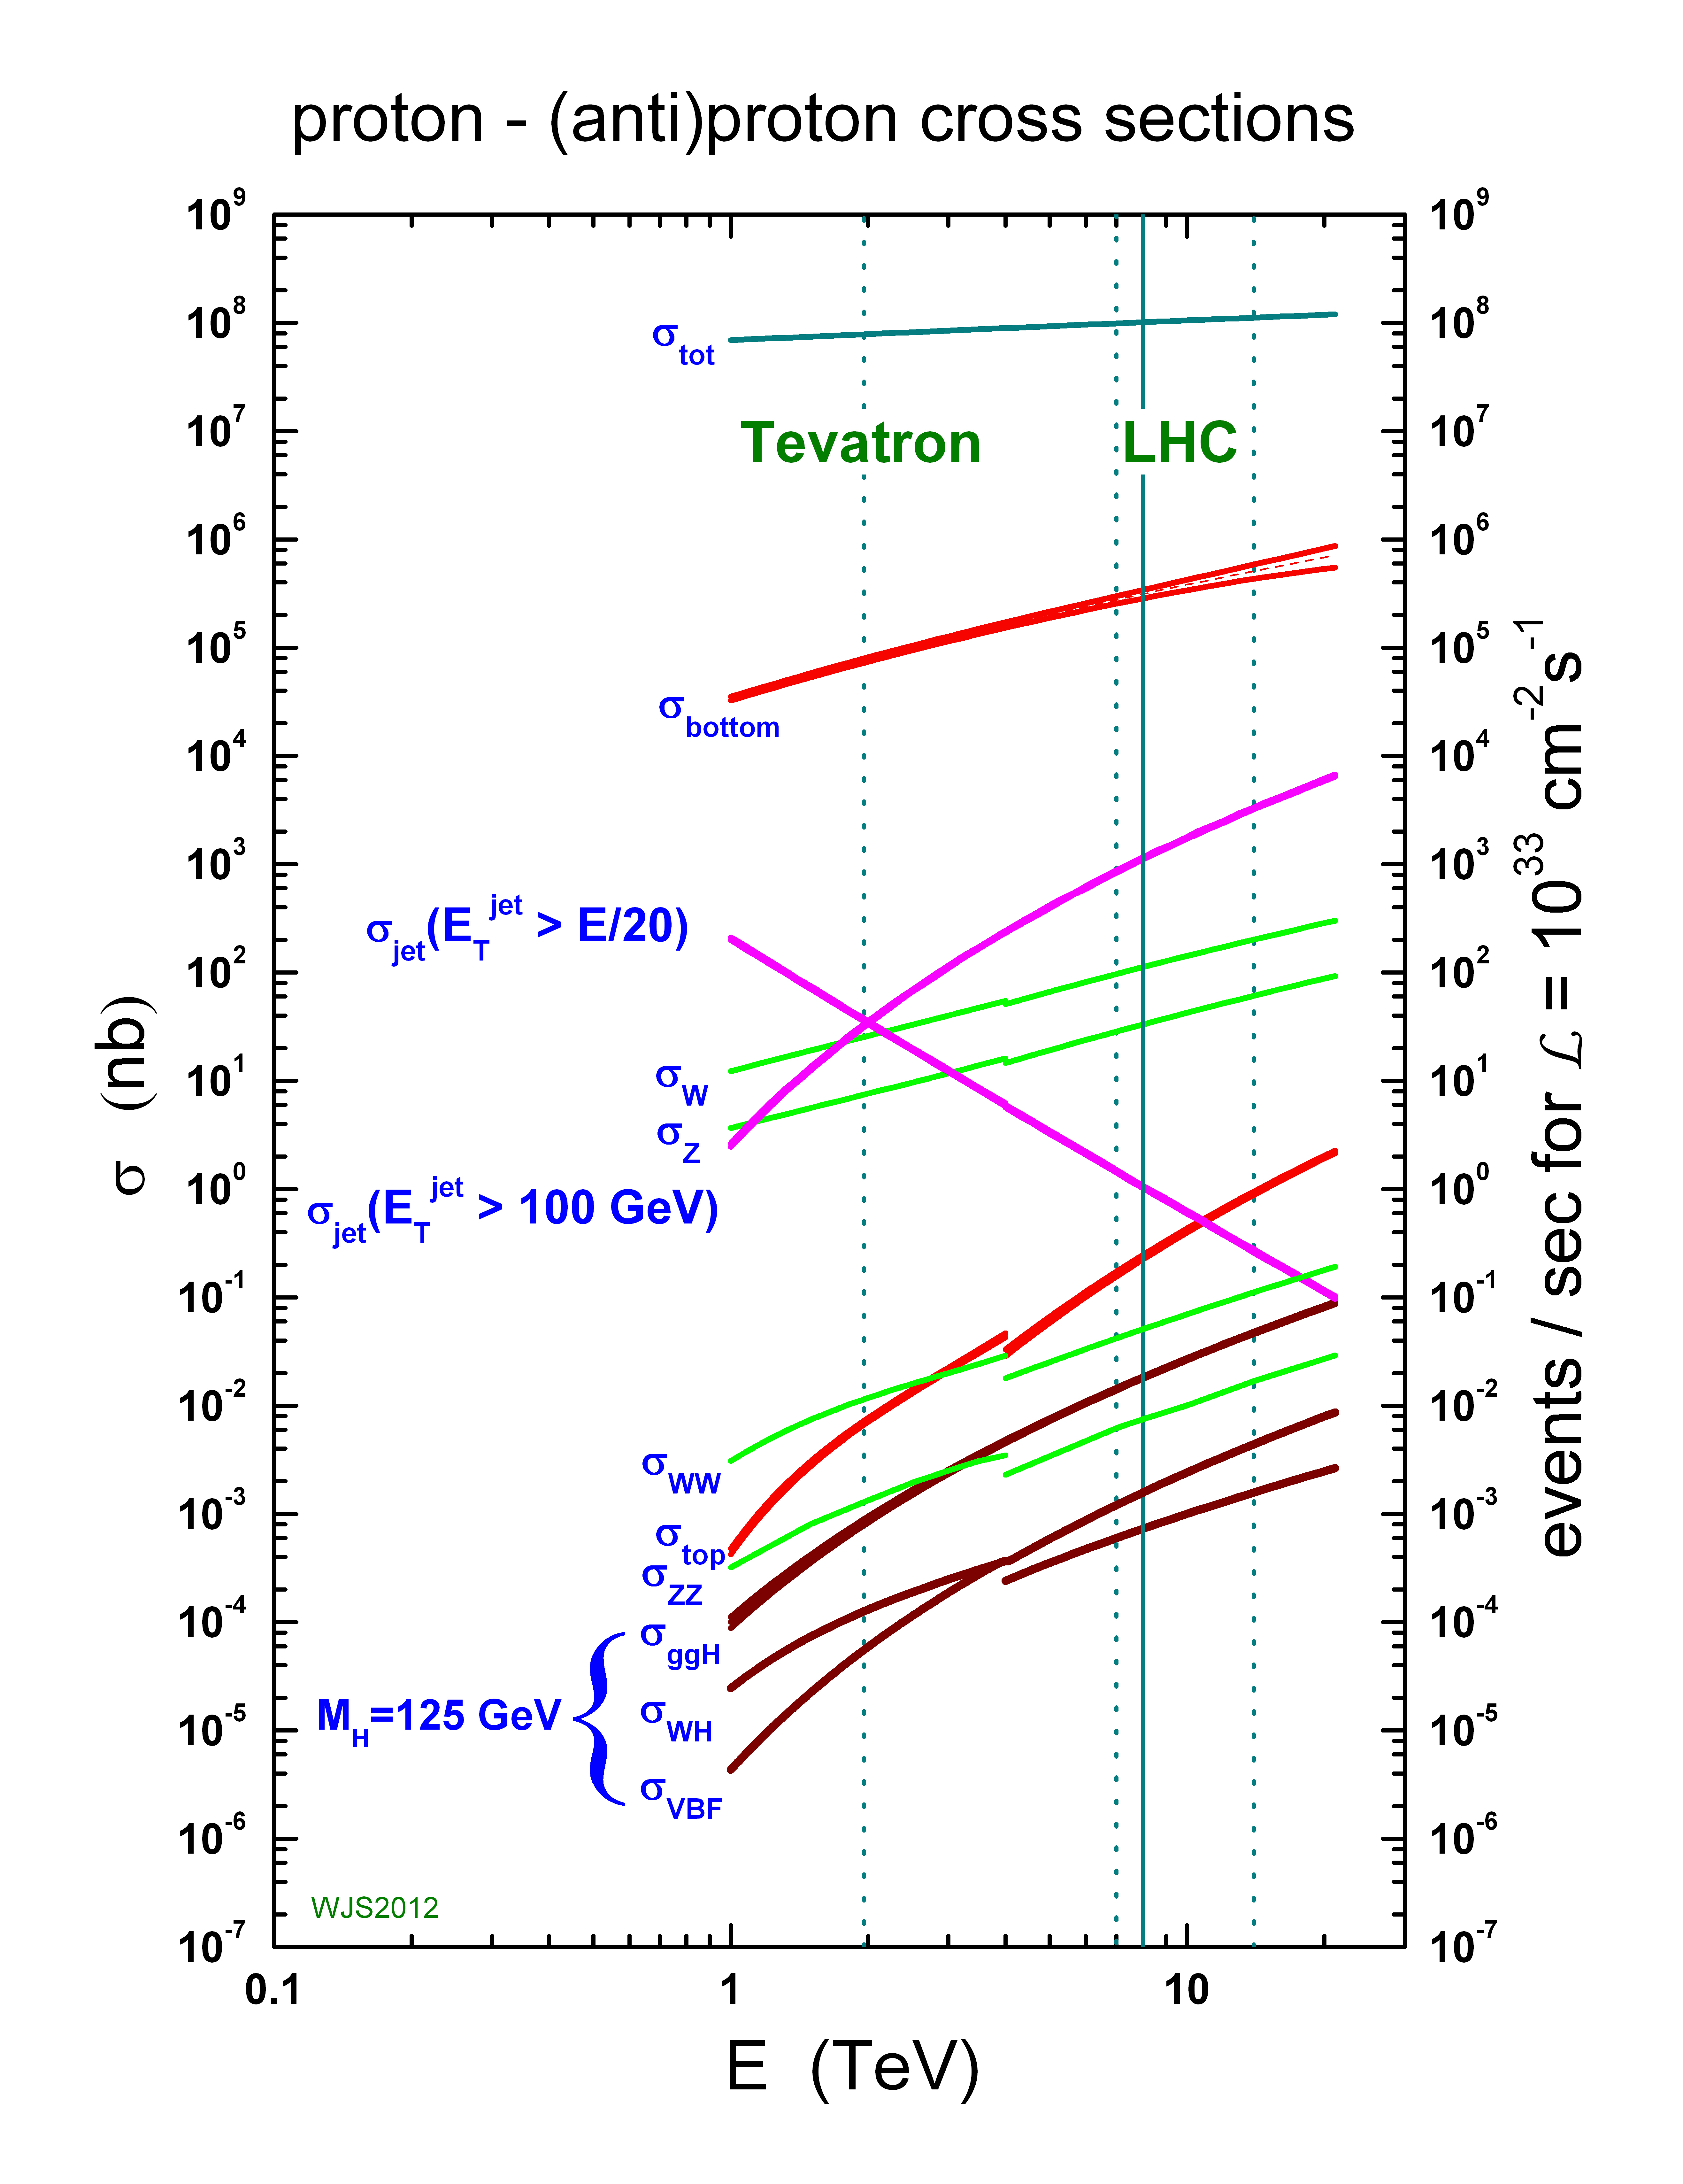
\includegraphics[width=.7\textwidth]{figures/lhc_decay_modes.jpg}
      \caption{Production Cross Sections for proton-proton collisions. Cross sections at center of mass energy less than 4 TeV are taken from proton-antiproton collision data at the Tevitron, which leads to some discontinuity for some types of electroweak boson production.}
      \label{fig:lhc_decay_modes}
    \end{figure}

    \begin{figure}[h!]
      \centering
      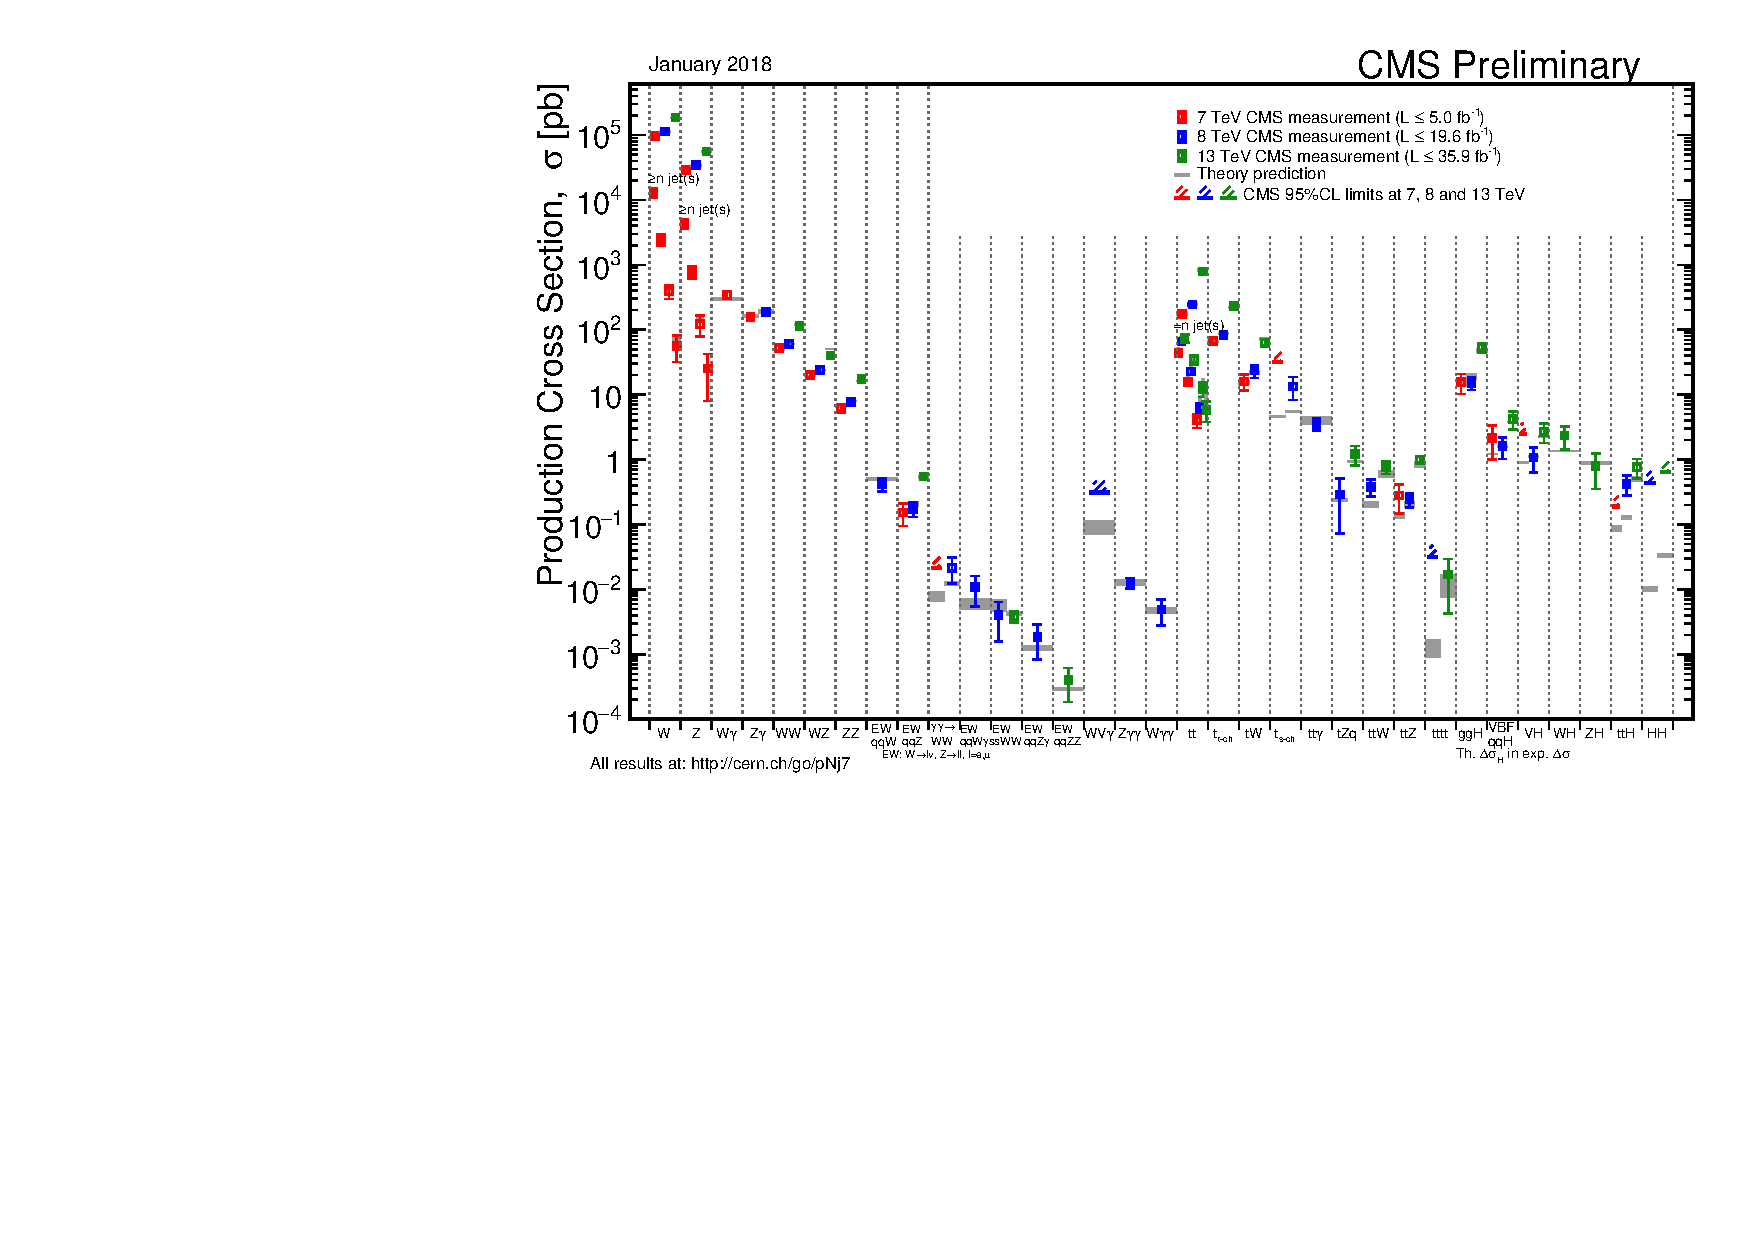
\includegraphics[width=.7\textwidth]{figures/cms_cross_sections.pdf}
      \caption{Cross sections measured by the CMS collaboration as of January 2018. Note that the cross section for Z+2 jets is close to the cross section for TTBar production. Additionally, note that for W and Z bosons, the cross section reduction in adding an additional jet is a factor between 5 and 10, consistent with the value of $\alpha_s$ at these energies. Taken from \cite{cms_results}}
      \label{fig:cms_cross_sections}
    \end{figure}

    \todo{Point out that there is very low chance for double scattering or two interesting interactions in one bunch crossing. 
    Point out cross section of Z boson, point out the NJets rule.
    Consider adding the other figure on my wall at the office. That way I can point out the njets rule and show the background composition with 2 jets.}

\section{The CMS Detector}
  
  The Compact Muon Solenoid (CMS) is a general purpose detector at the LHC. The detector is shown in figure \ref{fig:cms_detector}. It is the second largest detector at the LHC, weighing just under 15 kilotons. The envelope of the detector is a cylinder of radius 7.3 meters and length of 21.6 meters. The detector subsystems are embedded like an onion, sorted by what a particle produced at the interaction point would encounter traveling away from the beam pipe, the detector subsystems are as follows:

  \begin{enumerate}
    \item{Silicon Pixel Tracker}
    \item{Silicon Strip Tracker}
    \item{Electromegnetic Calorimeter}
    \item{Hadronic Calorimeter}
    \item{Superconducting Solenoid}
    \item{Muon Drift Tubes}
  \end{enumerate}

  The subsystems are broken into at least two regions. The \emph{barrel} region is the central part of the detector, and it is built of mostly of detection modules that are oriented parallel to the beam pipe, since particles traveling through this part of the detector have more transverse than longitudinal momentum. The \emph{end cap} contains modules oriented perpendicular to the beam pipe, since particles traveling through this part of the detector have more longitudinal momentum.

  \begin{figure}[h!]
    \centering
    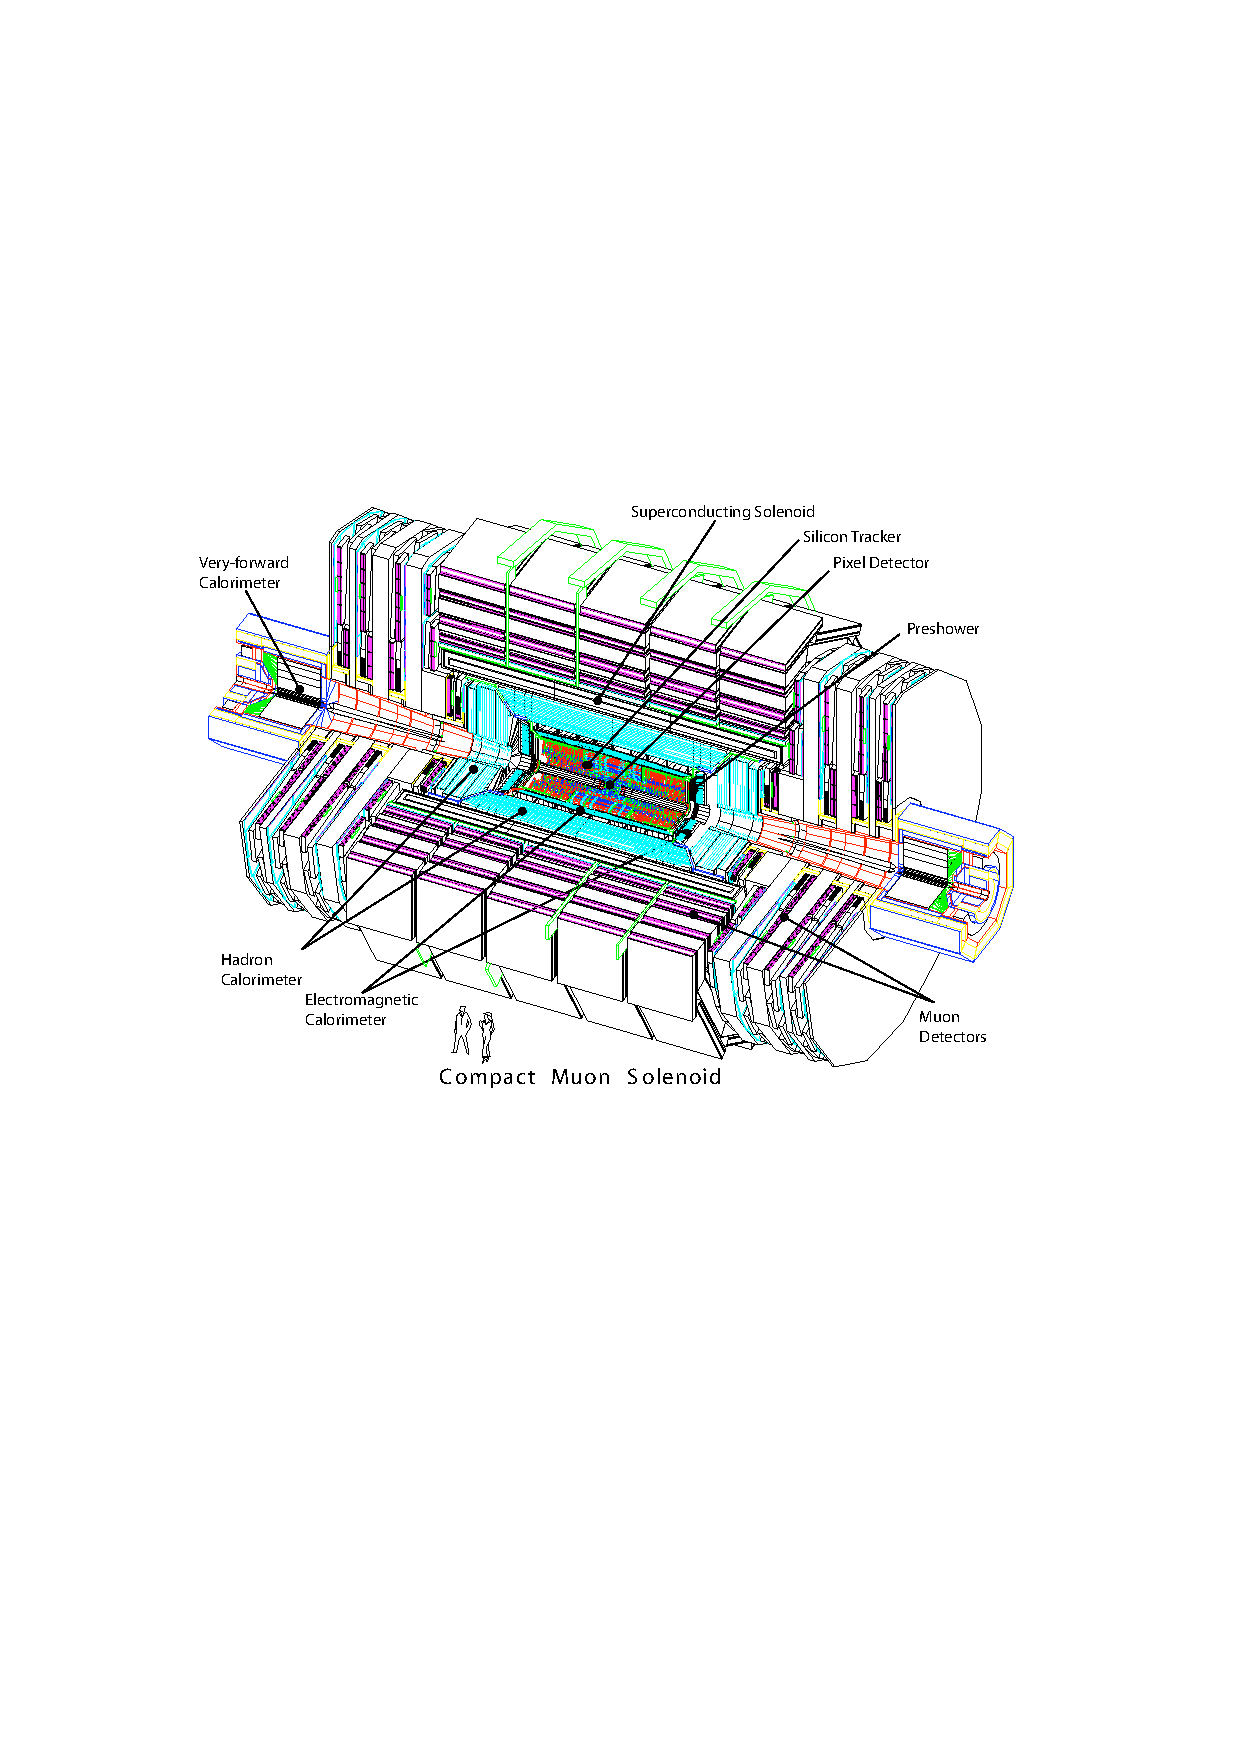
\includegraphics[width=.7\textwidth]{figures/cms_detector.pdf}
    \caption{A cutaway drawing of the Compact Muon Solenoid. Taken from the CMS TDR \cite{cms_tdr}.}
    \label{fig:cms_detector}
  \end{figure}

  As was shown in sec \ref{sec:what_gets_made}, most collisions at the LHC produce sprays of hadrons called jets, in fact the bulk of interactions are between gluons. However, more rare electroweak processes, such as the production of the higgs boson, can lead to the creation of leptons. Therefore, measuring the energy spectra of leptons is of central importance for CMS analyses searching for new physics coupled to the electroweak sector; this search is one such analysis. 

  The CMS detector needs to be able to identify charged leptons and distinguish their flavor in order to probe electroweak physics without hadronic backgrounds. The electron is a stable particle, and the muon has a lifetime long enough that it should make it through

  In order to measure the momentum of charged particles, a large magnetic field is applied by a superconducting solenoid that is placed between the hadronic calorimeter and the muon system. The solenoid creates a roughly constant 3.8 Tesla magnetic field parallel to the beam pipe in the region of the detector filled by the tracking system and calorimeters. This magnetic field will bend charged particles in accordance with the Lorentz force law and allow for a measurement of the particles momentum.

  CMS was designed with several physics goals in mind, from finding the Higgs boson, to searches for dark matter and supersymmetry. The technical design report (TDR) \cite{cms_tdr} summarizes the physics and design goals for the detector. A short list follows:

  \begin{enumerate}
    \item The search for the Higgs boson, specifically in the dimuon and diphoton channel\footnote{the diphoton channel was where it ultimately was found}. This created a need for excellent muon and photon energy resolution and isolation. These requirements justify the advanced muon system and ECAL. Additionally searching for the Higgs in the $b\bar{b}$ and $\tau \bar{\tau}$ channels created the requirement for good offline b-tagging and $\tau$-tagging capabilities, largely regulated by tracker resolution.
    \item The search for supersymmetric (SUSY) particles. The main motivation for these searches is often in the context of R-parity conserving SUSY due to the natural dark matter candidate they provide as described in section \ref{sec:r-parity}. Dark particles leave momentum imbalance in the detector, so there is 
    \item The search for new massive vector bosons, typically dubbed a Z' search. Here dilepton (electron and muon) energy resolution are again of the paramount importance.
    \item The search for extra dimensions. The phenomenology of these models is very broad, but signatures can include all massive standard model particles and gravitons which leave a \MET signature.
    \item Measurements furthering the precision Standard Model parameters. The production of top quarks is enhanced at the LHC compared to any previous colliders due to their large mass, even compared to the TeV scale. Top quarks almost always decay to b-quarks which means the LHC is also a b-factory.
    \item In addition to proton-proton collisions, the LHC also collides lead ions which probe the thermodynamic properties of quantum chromodynamics (QCD), the theory of the strong nuclear force. These collisions typically produce hadronic jets and their \pt spectrum is of interest due to observations at RHIC \cite{QCD_collider_physics}.
  \end{enumerate}

  \subsection{Coordinate System}
    Throughout this document, a standard coordinate system is used, this system is a cylindrical coordinate system with the $z$ axis oriented along the beam pipe. $z=0$ is situated at the mid-point of the detector, 10.8 m from either edge. The $\theta = 0$ direction points toward the Jura mountains, with $\theta = 90^\circ$ pointing straight upwards, away from the center of the earth. 

    Rather than $\theta$, we use the pseudorapidity, $\eta = - \ln \left( \tan\left(\frac{\theta}{2}\right)\right)$. $\eta = 0$ corresponds to $\theta = 90^\circ$ and $\eta$ grows to infinity as $\theta$ goes to 0. The benefit of using $\eta$ is that differences in $\eta$, $\Delta \eta$, between two particles are approximately invariant under Lorentz boosts along the beam axis, whereas differences in $\theta$ are not. The extent to which $\Delta \eta$ is equal in different reference frames is regulated by the mass of the particles, with equality achieved in the case where the mass to momentum ratio of the particles goes to 0, i.e. the high energy limit.\footnote{Pages 6-8 in reference \cite{psuedorapidity} shows that differences in rapidity are Lorentz invariant and that psuedorapidity and rapidity are equal in the high energy limit} The detector's fiducial area corresponds to about $\abs{\eta} < 2.4$, which is about $10^\circ$ off of the beampipe. The positive $x$ axis is defined as pointing to the center of the circle outlined by the LHC, and the positive $y$ axis points towards the sky. The $\phi$ direction is the angle from the positive $x$ axis to the positive $y$ axis. Figure \ref{fig:cms_coordinates} shows this information visually.

    \begin{figure}[h!]
      \centering
      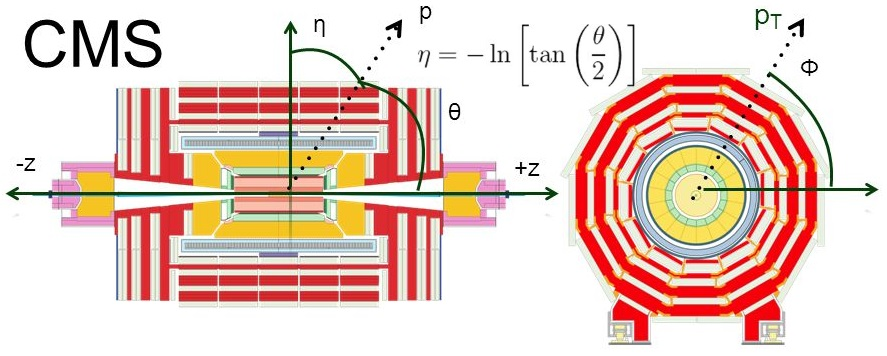
\includegraphics[width=.7\textwidth]{figures/cms_coordinates.jpg}
      \caption{Cross sectional and transverse views of the CMS detector with $\eta$, $\phi$, and $\theta$ coordinates shown. Taken from \cite{cms_coordinates}.}
      \label{fig:cms_coordinates}
    \end{figure}

  \subsection{The Inner Tracker} \label{sec:inner_tracker}
    The inner tracker is the closest part of the CMS detector to LHC beamline and interaction point where protons collide. \cite{cms_jinst} It surrounds the interaction point with a length of 5.8m and radius of 1.25m. The purpose of the system is to track charged particles to their vertex and measure the momentum of charged particles via the saggita in the particle arc due to the magnetic field. The entire active detection area of the inner-tracker system is made of silicon, but can be broken into 2 main subsystems:

    \begin{enumerate}
      \bitem{pixel detectors} The innermost part of the tracker system is a pixel-based detector composed of 1,440 thin modules, of cross section $100 \times 150 \mu$m$^2$, capable of measuring hits with fine granularity in 3 dimensions. This subsystem's main purpose is to aid in vertex reconstruction.
      \bitem{strip detectors} The outer part of the inner tracker is composed of 15,148 strip modules. The main purpose of this subsystem is to track charged particles from the vertex into the ECAL and also to give one measure of their momentum.
    \end{enumerate}

    Silicon detectors work on the principle of semi-conduction. When a charged particle passes through the material, electrons are kicked into the conduction band and drift, due to a bias voltage applied across the sample, towards electronics attached to the material that record the current. Because silicon has a relatively small band gap, the entire tracking system needs to be kept at low temperature, approximately $-10^\circ$ C, in order to keep the electrons stationary in the valence band in the presence of the bias voltage.

    The tracker geometry is shown in figure \ref{fig:strip_tracker_geometry}. The pixel detectors are the closest to the beampipe and consist of 3 layers in the barrel region and 2 annuli in the endcap region. The three barrel layers are positioned in concentric cylinders about the beampipe at radii of 4.4 cm, 7.3 cm, and 10.2 cm respectively. The endcap annuli are placed at $\abs{z} = 34.5 $cm and 46.5 cm respectively and have an inner radius of 6 cm and an outer radius of 15 cm. The strip tracker consists of an inner barrel region (TIB), an outer barrel region (TOB), and an inner disk region (TID) in the barrel, and two endcap regions (TEC +/-). 

    \begin{figure}[h!]
      \centering
      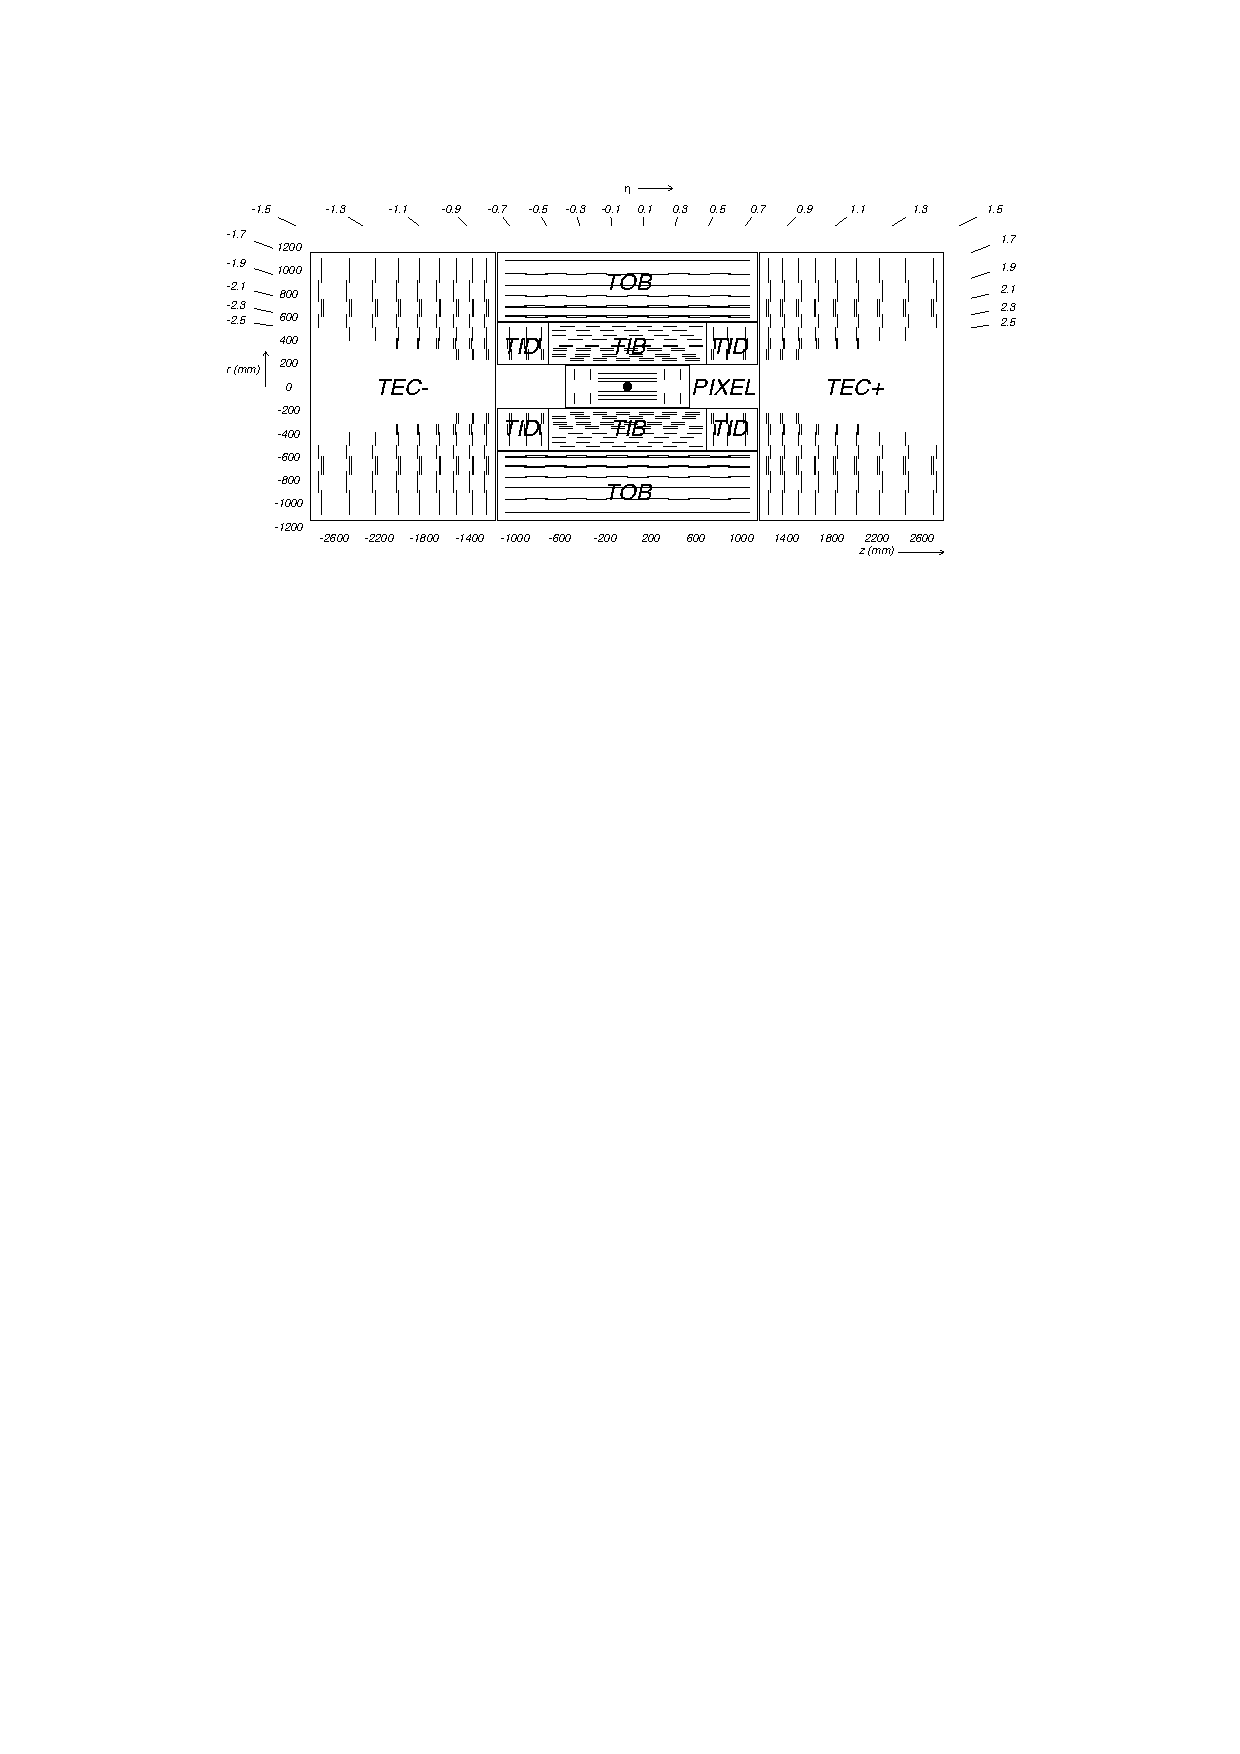
\includegraphics[width=.7\textwidth]{figures/cms_tracker_schematic.pdf}
      \caption{Schematic view of the CMS inner tracking system. Notice the detectors only cover $\abs{\eta}$ ranges less than 2.5 and that particles traveling near $\abs{\eta}=1.5$ pass through the most material. Taken from \cite{cms_jinst}.}
      \label{fig:strip_tracker_geometry}
    \end{figure}

    Because one of the goals of the tracking system is to obtain a measure of momentum by tracking the natural motion of particles through space in a magnetic field, it is important that the interactions between charged particles and the tracking system do not change the motion, and likewise the energy, of the particles dramatically. For particles other than the electron and photon, the silicon tracker has mostly negligible effects on the energy as the amount of bremsstrahlung is inversely proportional to the mass of the particle to approximately the 6th power;\footnote{This can be seen in the classical theory of bremsstrahlung radiation as described in \cite[pg. 464, eq. 11.75]{griffiths_em} by replacing the Lorentz factor $\gamma$ with $\frac{E}{mc^2}$. In the case of an acceleration in an orthogonal direction, $\gamma^6 \to \gamma^4$.} their main energy loss mechanism is through ionization.\cite[sec. 33.2]{PDG} However, for the electron and the photon, interaction with the tracker can cause bremsstrahlung radiation and pair production respectively.

    To understand the magnitude of these effects, it is typical to look at the number of radiation lengths\footnote{taken to be the distance at which a high energy electron is expected to lose $\frac{1}{e}$ of its energy \cite[sec 34.4.2]{PDG}, or $\frac{7}{9}$ the mean free path for a high energy photon.} of material in the tracker. The ``material budget" of the tracker is shown in figure \ref{fig:tracker_material_budget}. Due to the large amount of non-sensitive material in the range $\abs{\eta} \in [1.4,1.6]$, leptons for this analysis are not considered in that range, as is explained in section \ref{sec:dilepton_selection}. As can be seen in the figure, many $\eta$ values correspond to high probability of radiation and pair production for electrons and photons respectively. We will explain in section \ref{sec:particle_flow} how the momentum of these types of particles is reconstructed given these issues.

    \begin{figure}[h!]
      \centering
      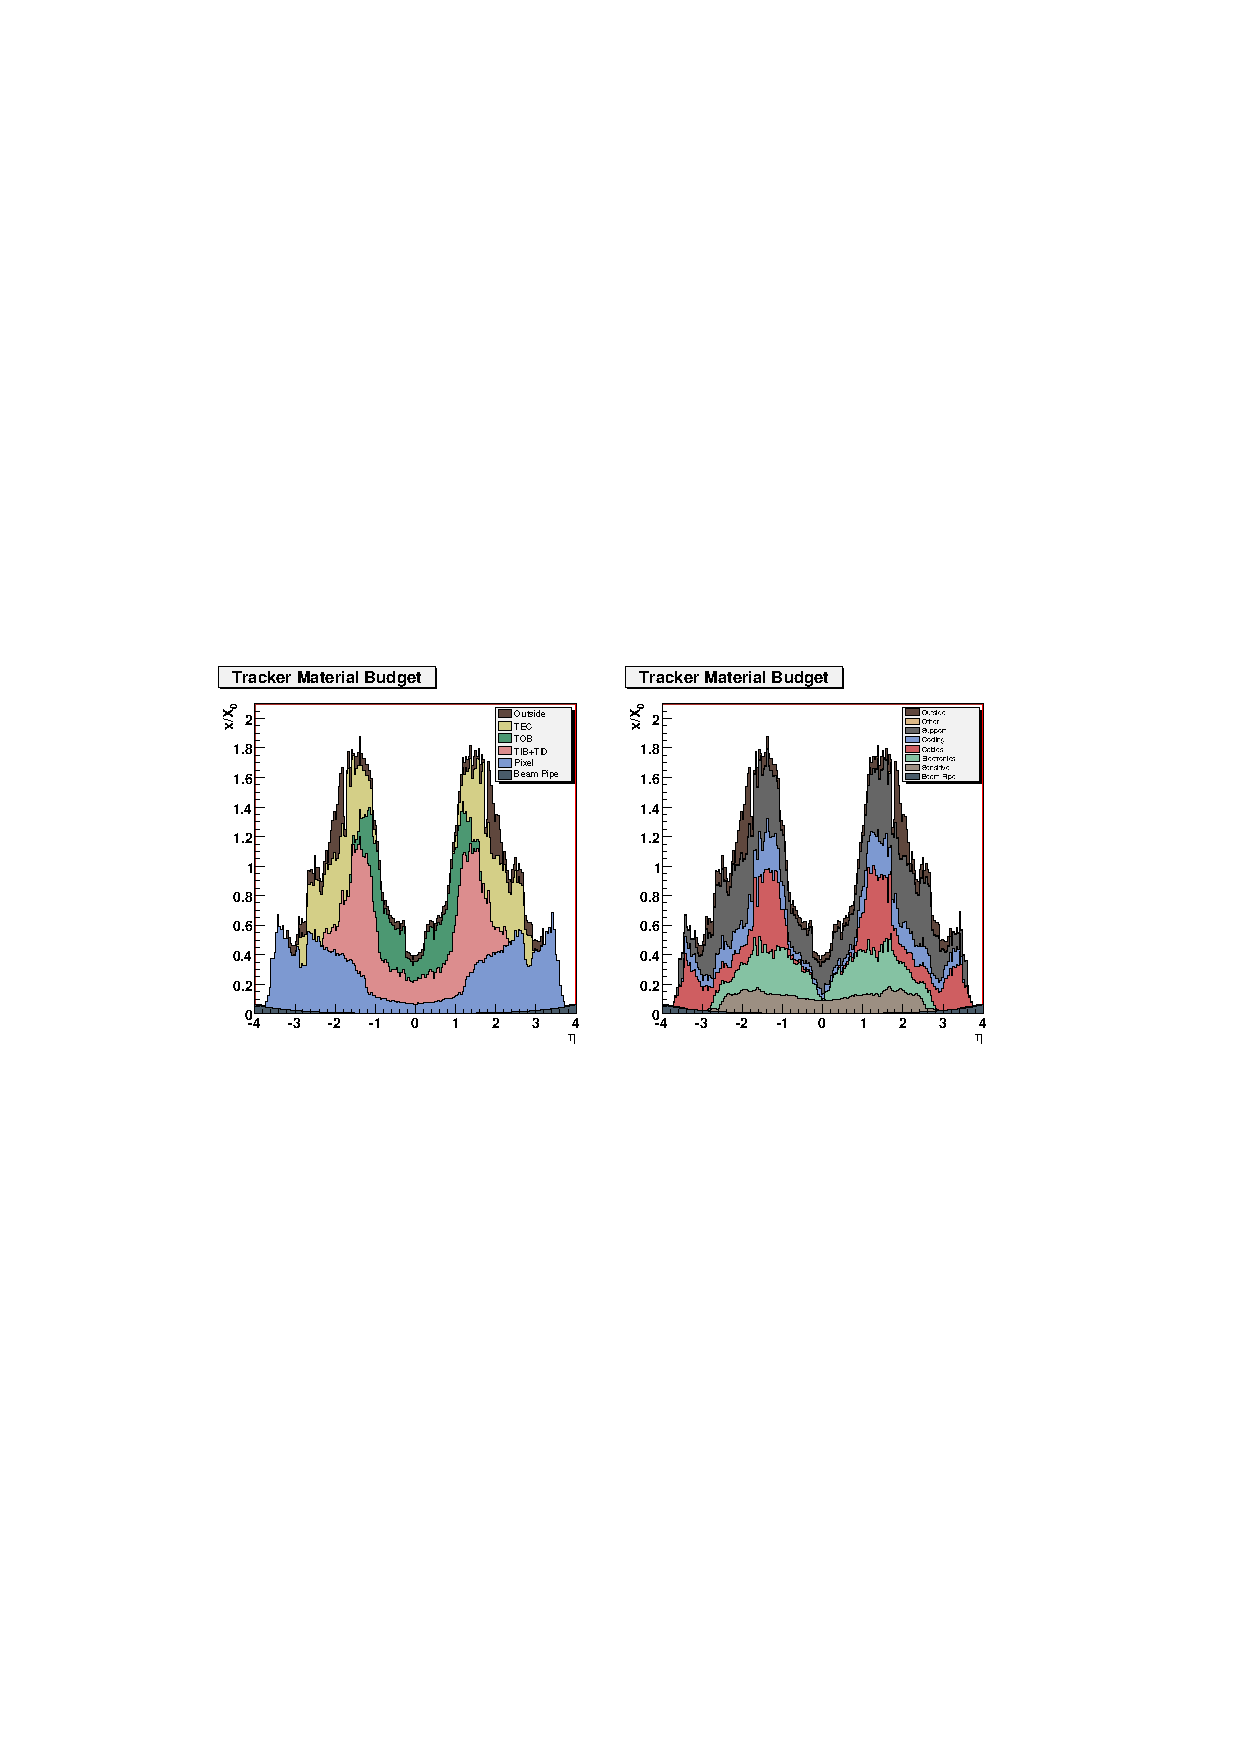
\includegraphics[width=.9\textwidth]{figures/cms_tracker_material_budget.pdf}
      \caption{The material budget of the tracking system in radiation lengths. On the left, the material is broken down by tracker subsystem, on the right it is broken down by the type of component. As can be seen on the right plot, a large amount in non-sensitive material, like cables and support structure, is found near $\abs{\eta}=1.5$. For this reason, leptons in this analysis are not used if they are found in the window $\abs{\eta} \in [1.4,1.6]$. Taken from \cite{cms_jinst}.}
      \label{fig:tracker_material_budget}
    \end{figure}

  \subsection{The Electromagnetic Calorimeter} \label{sec:ECAL}
    The CMS Electromagentic Calorimeter (ECAL) is a nearly hermetic and homogeneous cylinder made of lead tungstate (PbWO$_4$) crystals with attached light measuring devices. The crystals are ``truncated pyramids", roughly rectangles of approximately 23 centimeters in length that taper slightly, from 26x26 mm$^2$ to 22x22 mm$^2$ in the barrel\cite[pg. 4]{cms_ecal}, to accommodate the curved shape of the ECAL in the $\phi$ direction and the angle at which the crystals are oriented to face the interaction point.\footnote{the crystals have a 3$^\circ$ angle with respect to the line that connects their incident face to interaction point in both the $\eta$ and $\phi$ directions to allow for better coverage of the fiducial volume.} Schematic views of the ECAL can be seen in figures \ref{fig:ecal_xsec} and \ref{fig:ecal_cutaway}. As can be seen in the figures, the calorimeter is broken into two physical sections, the barrel region (EB) and the endcap region (EE). The preshower disk in front of the endcap region is immaterial for this search, but is there to help distinguish between neutral pions converting to a di-photon pair with small angle separation from a single high energy photon. 

    \begin{figure}[h!]
      \centering
      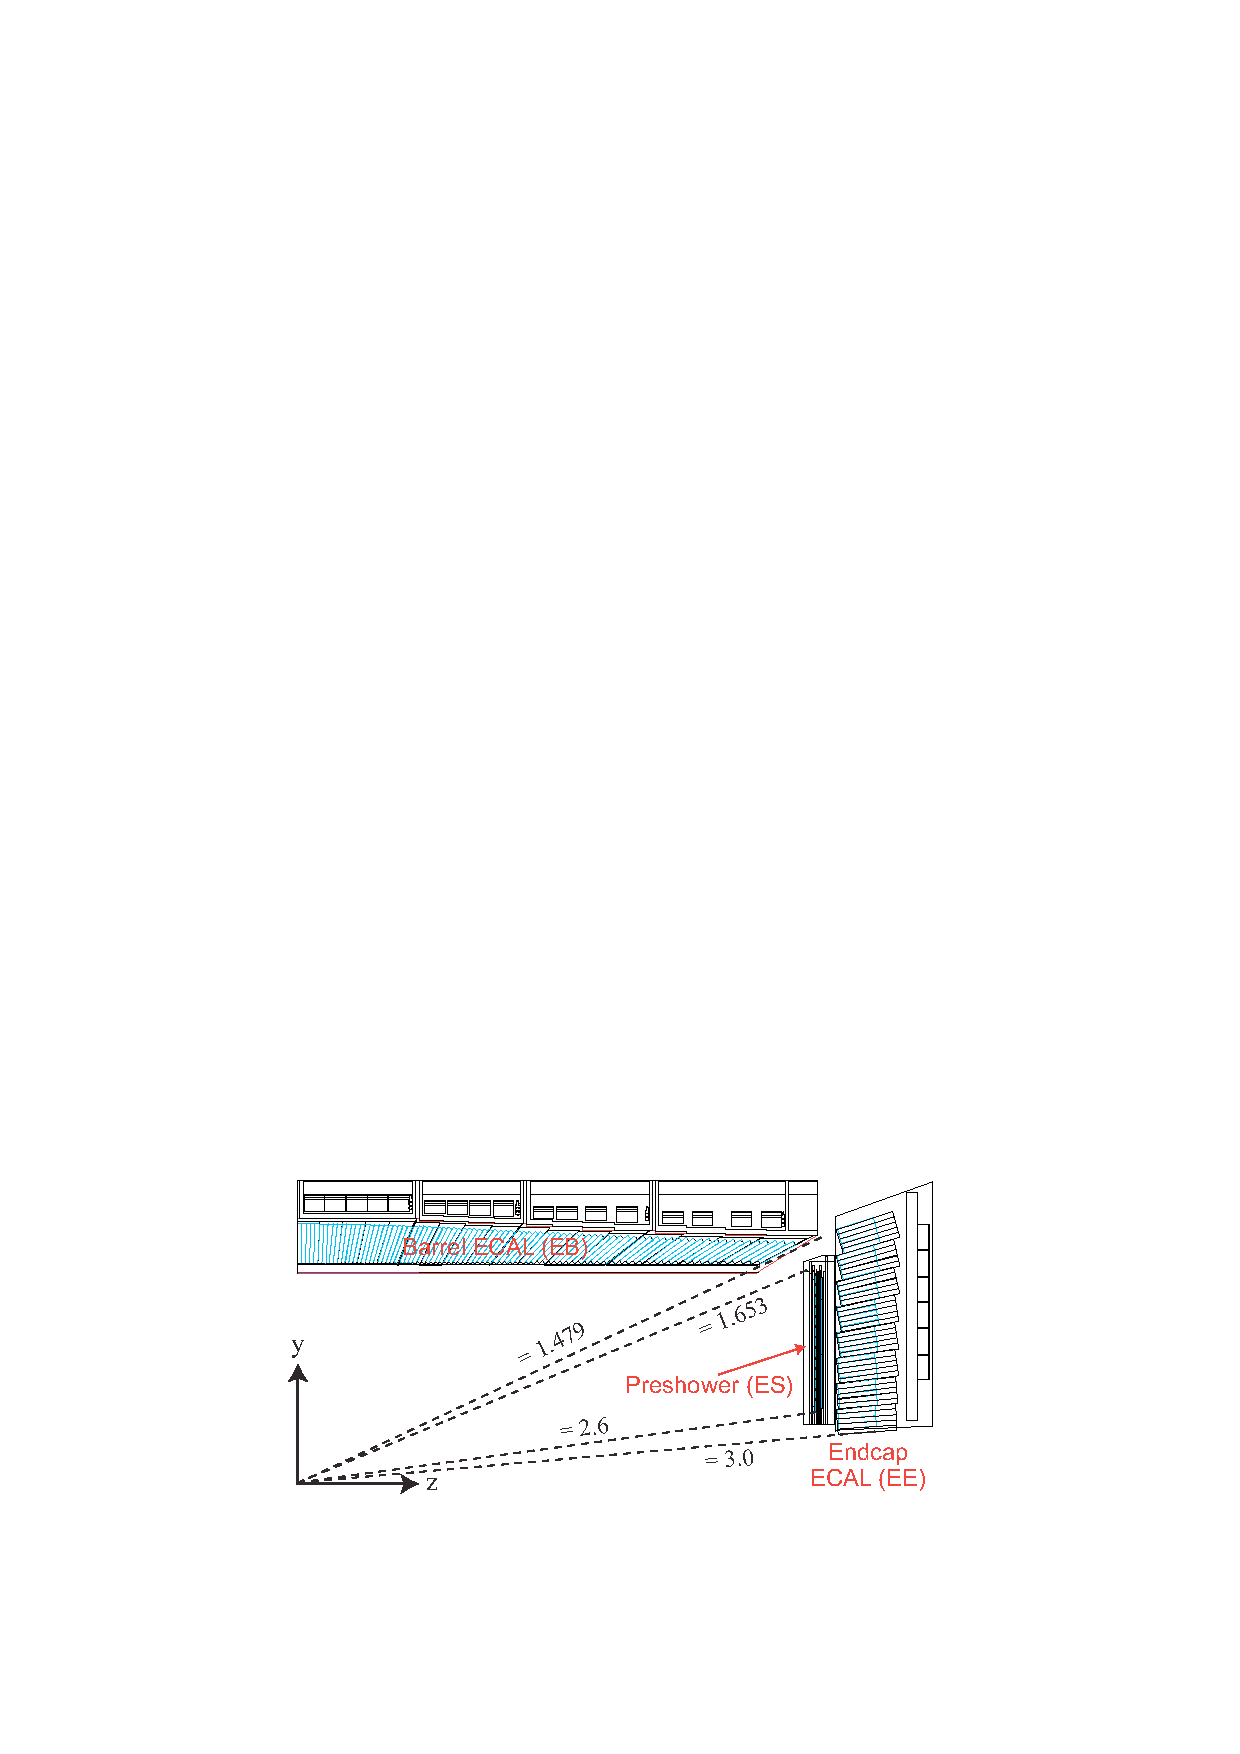
\includegraphics[width=.9\textwidth]{figures/cms_ecal_xsec.pdf}
      \caption{A cross sectional view of the electromagnetic calorimeter on the CMS detector. Notice the geometry of the crystals the transition region near $\abs{\eta} = 1.5$. Taken from \cite{cms_tdr}.}
      \label{fig:ecal_xsec}
    \end{figure}

    \begin{figure}[h!]
      \centering
      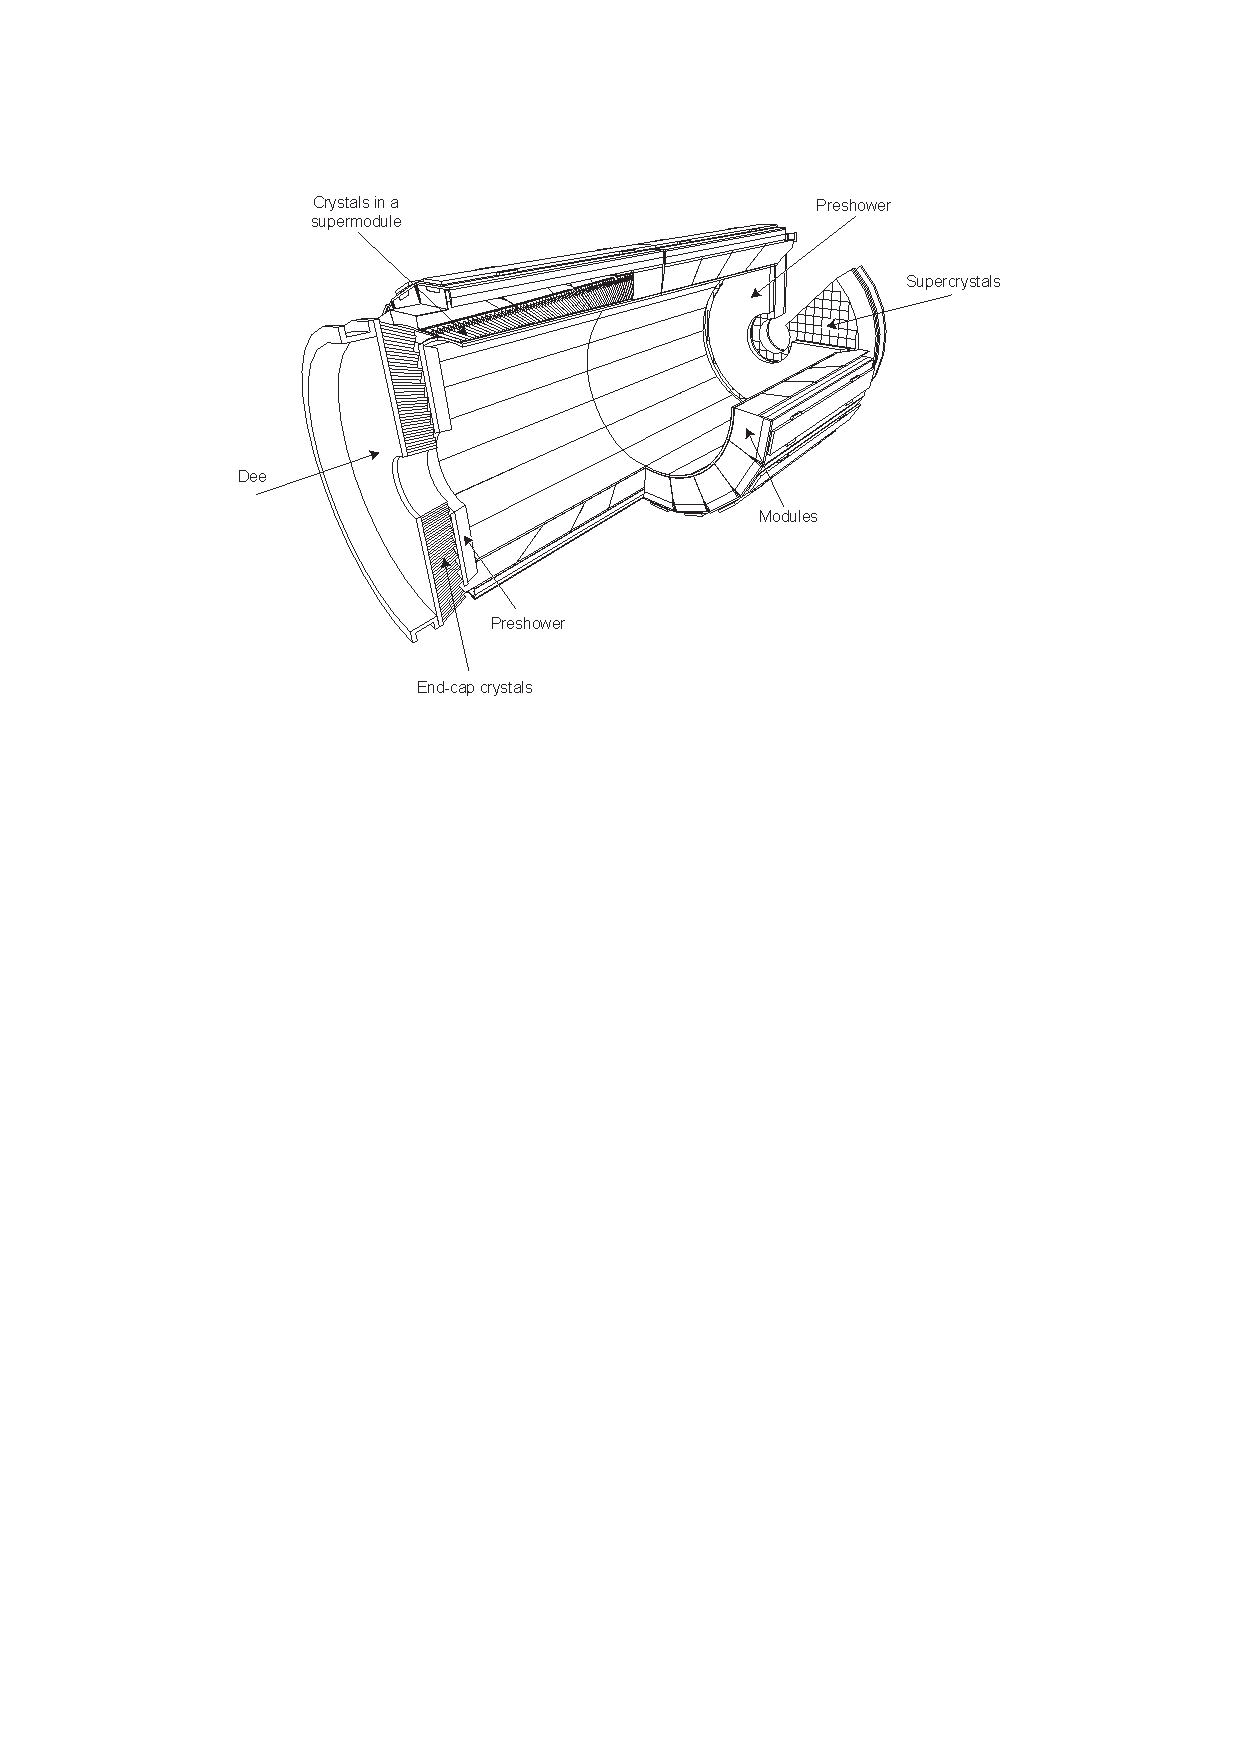
\includegraphics[width=.9\textwidth]{figures/cms_ecal.pdf}
      \caption{A cutaway of the electromagnetic calorimeter on the CMS detector. Taken from \cite{cms_jinst}.}
      \label{fig:ecal_cutaway}
    \end{figure}

    The purpose of the ECAL is essentially to give the most important measure of energy for electrons and photons. As explained in the previous section, the dynamics of electrons in material are quite distinct from heavier charged particles in material, the next lightest being a muon. Typical muon deposits in the ECAL are roughly 300 MeV\cite{muon_stopping_power}, whereas electrons under 500 GeV tend to have almost all of their energy absorbed by the ECAL\cite[sec. 4.10]{cms_jinst}. This is to say that charged particles heavier than an electron tend to pass right through the ECAL with little disturbance. \todo{Is this actually correct? Should I have a section somewhere where I describe charged particle interactions with matter?}

    The ECAL operates on the principle of scintillation\cite[ch. 7]{leo_detectors}, and makes use of the fast scintillation time (80\% of light emitted within 25 ns), high stopping power, and consequently small Moli\`ere radius of lead tungstate. The lead tungstate crystals have a length which corresponds to approximately 25 radiation lengths, this ensures that almost all of the energy carried by a high energy photon or electron will be radiated. The small Moli\`ere radius allows for good spacial resolution of energy deposits. \cite[pg. 90]{cms_jinst} Two things happen when an electron or photon is incident on one of the crystals:

    \begin{enumerate}
      \item A cascade of electrons, positrons, and photons is created. This is due to the effects discussed in the previous section, photons will pair produce electron-positron pairs. Electrons and positrons undergo bremsstrahlung radiation in material creating high energy photons. The result is that these processes feedback on each other and the multiplicity of particles explodes in the material creating an ``electromagnetic shower". A hypothetical shower imposed on an ECAL crystal is shown in figure \ref{fig:ecal_crystal}.

      \item Scintillation light is emitted by the lead tungstate due to interactions with charged particles and the light captured by the photo detectors attached to the crystal.
    \end{enumerate}

    \begin{figure}[h!]
      \centering
      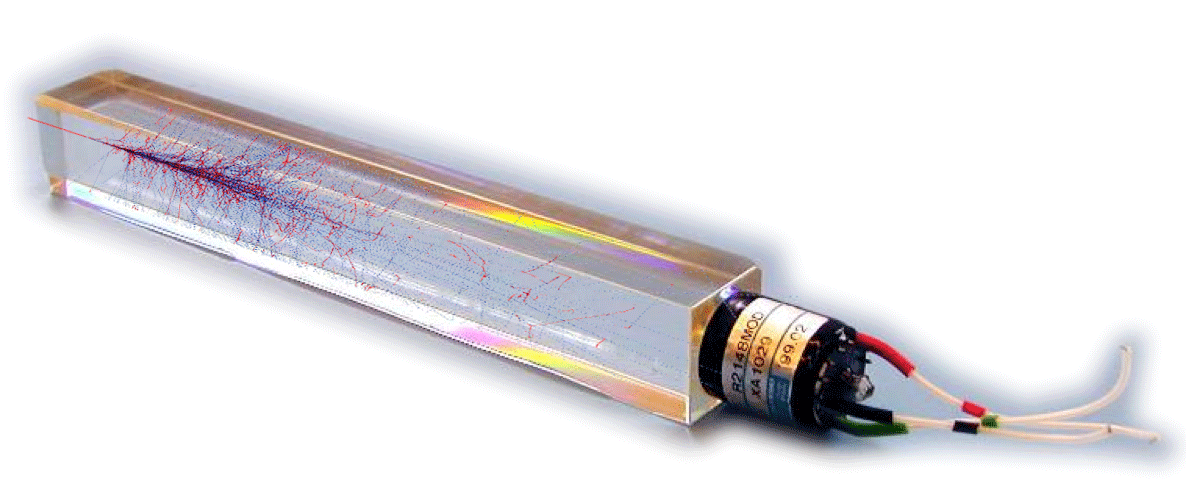
\includegraphics[width=.5\textwidth]{figures/cms_ecal_crystal_shower.png}
      \caption{A lead tungstate crystal from the CMS ECAL endcap region with a vacuum phototriode attached. A hypothetical shower from an electron is superimposed on the image. Taken from \cite{ecal_crystal}.}
      \label{fig:ecal_crystal}
    \end{figure}

    From the amount of scintillation light, the energy of the incident particle can be reconstructed with high resolution. Figure \ref{fig:ecal_resolution} shows the energy measured using a 5x5 grid of ECAL crystals for 120 GeV electrons. From the figure, we can see that the ECAL energy resolution is excellent for electrons in this range, the standard deviation of the energy measurement being 1-2\% of the energy.

    \begin{figure}[h!]
      \centering
      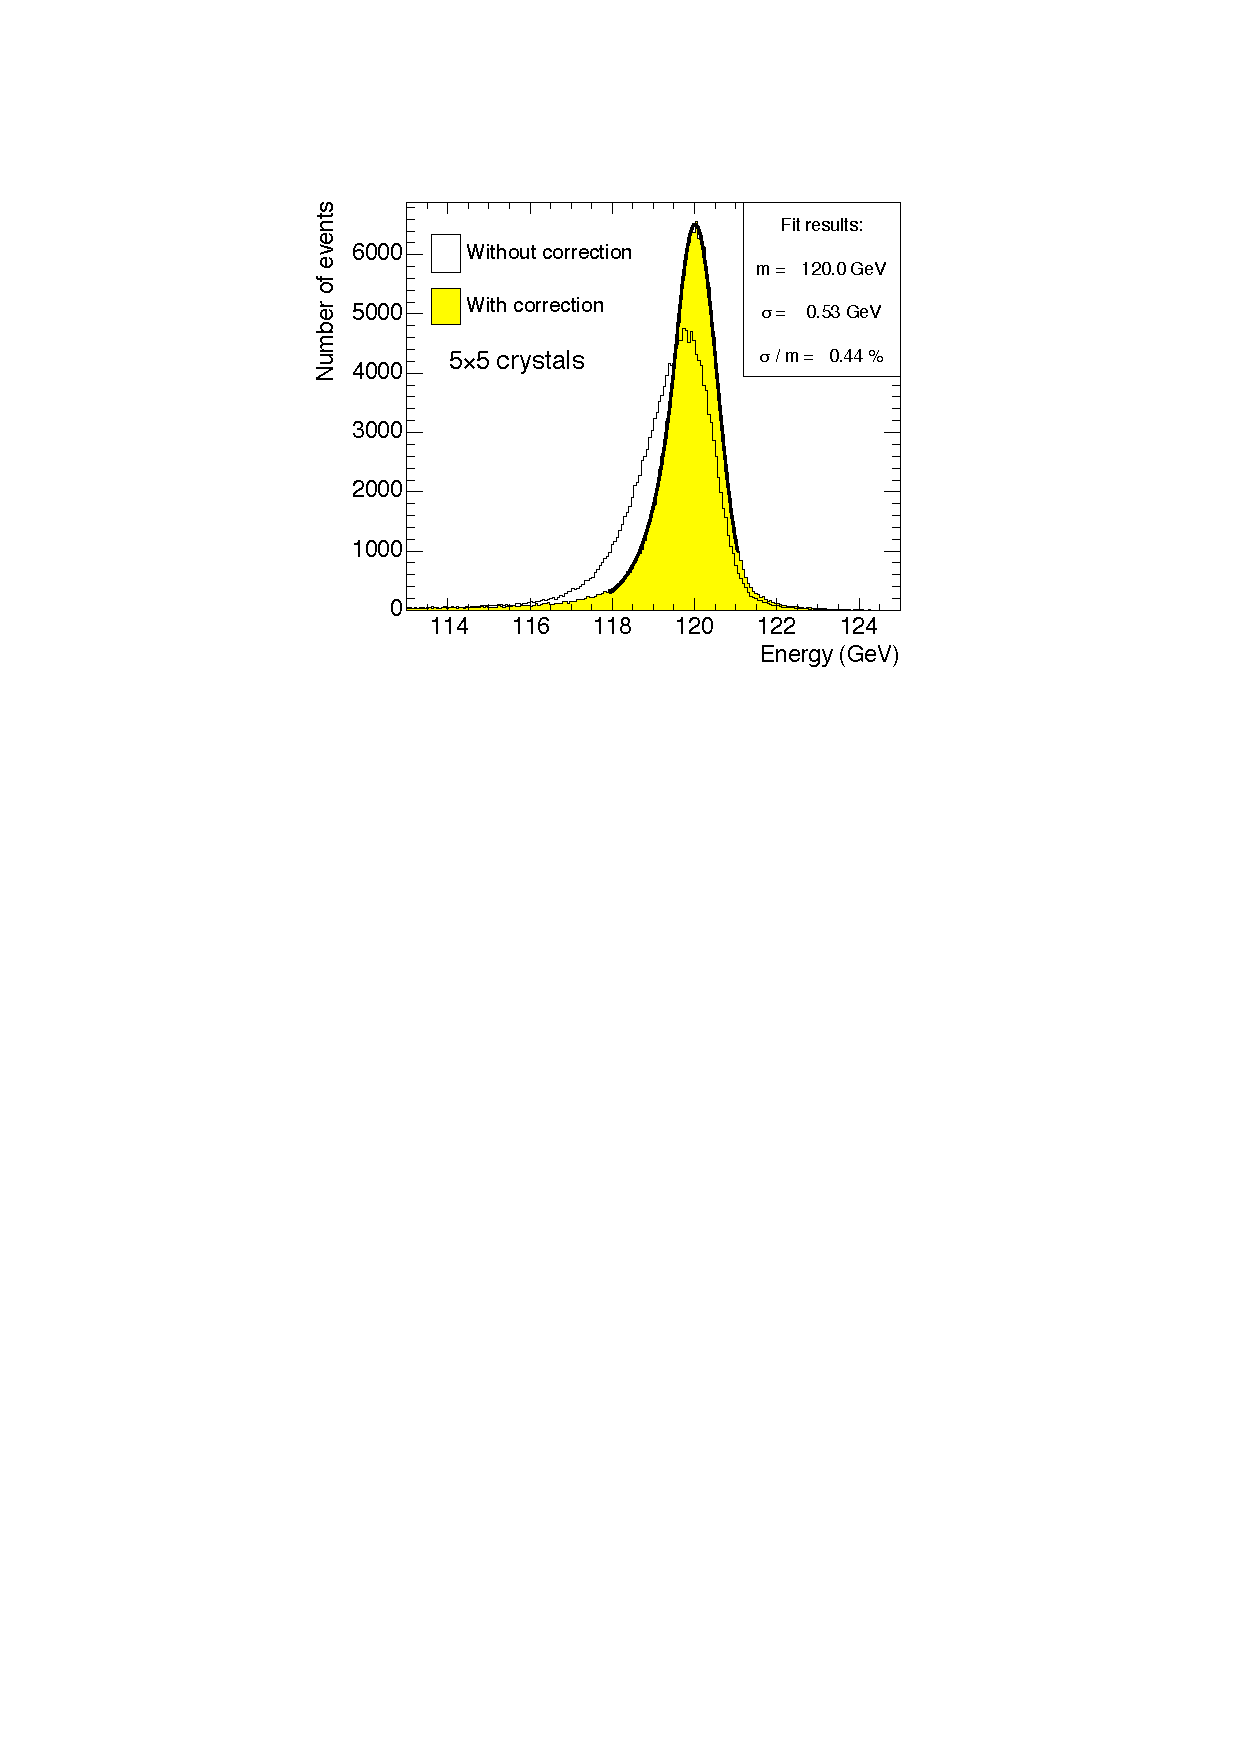
\includegraphics[width=.7\textwidth]{figures/ecal_resolution.pdf}
      \caption{The energy measured from 120 GeV electrons taken from a 5x5 grid of ECAL crystals. Taken from \cite{cms_jinst}.}
      \label{fig:ecal_resolution}
    \end{figure}

    \todo{What happens to the light that that doesn't pair produce? Is that also picked up by the photo diode? Also, why does the light always go forward, momentum only?}

  \subsection{The Hadronic Calorimeter}
    The CMS Hadronic Calorimeter (HCAL) is a sampling calorimeter made of interleaved layers of dense absorber metals with plastic scintillator material. The purpose of this subsystem is to measure the energy of the hadrons and massive charged particles that make up jets. The measurement of these objects are of particular importance for the reconstruction of \MET, which is a central event-level object in this analysis.

    \begin{figure}[h!]
      \centering
      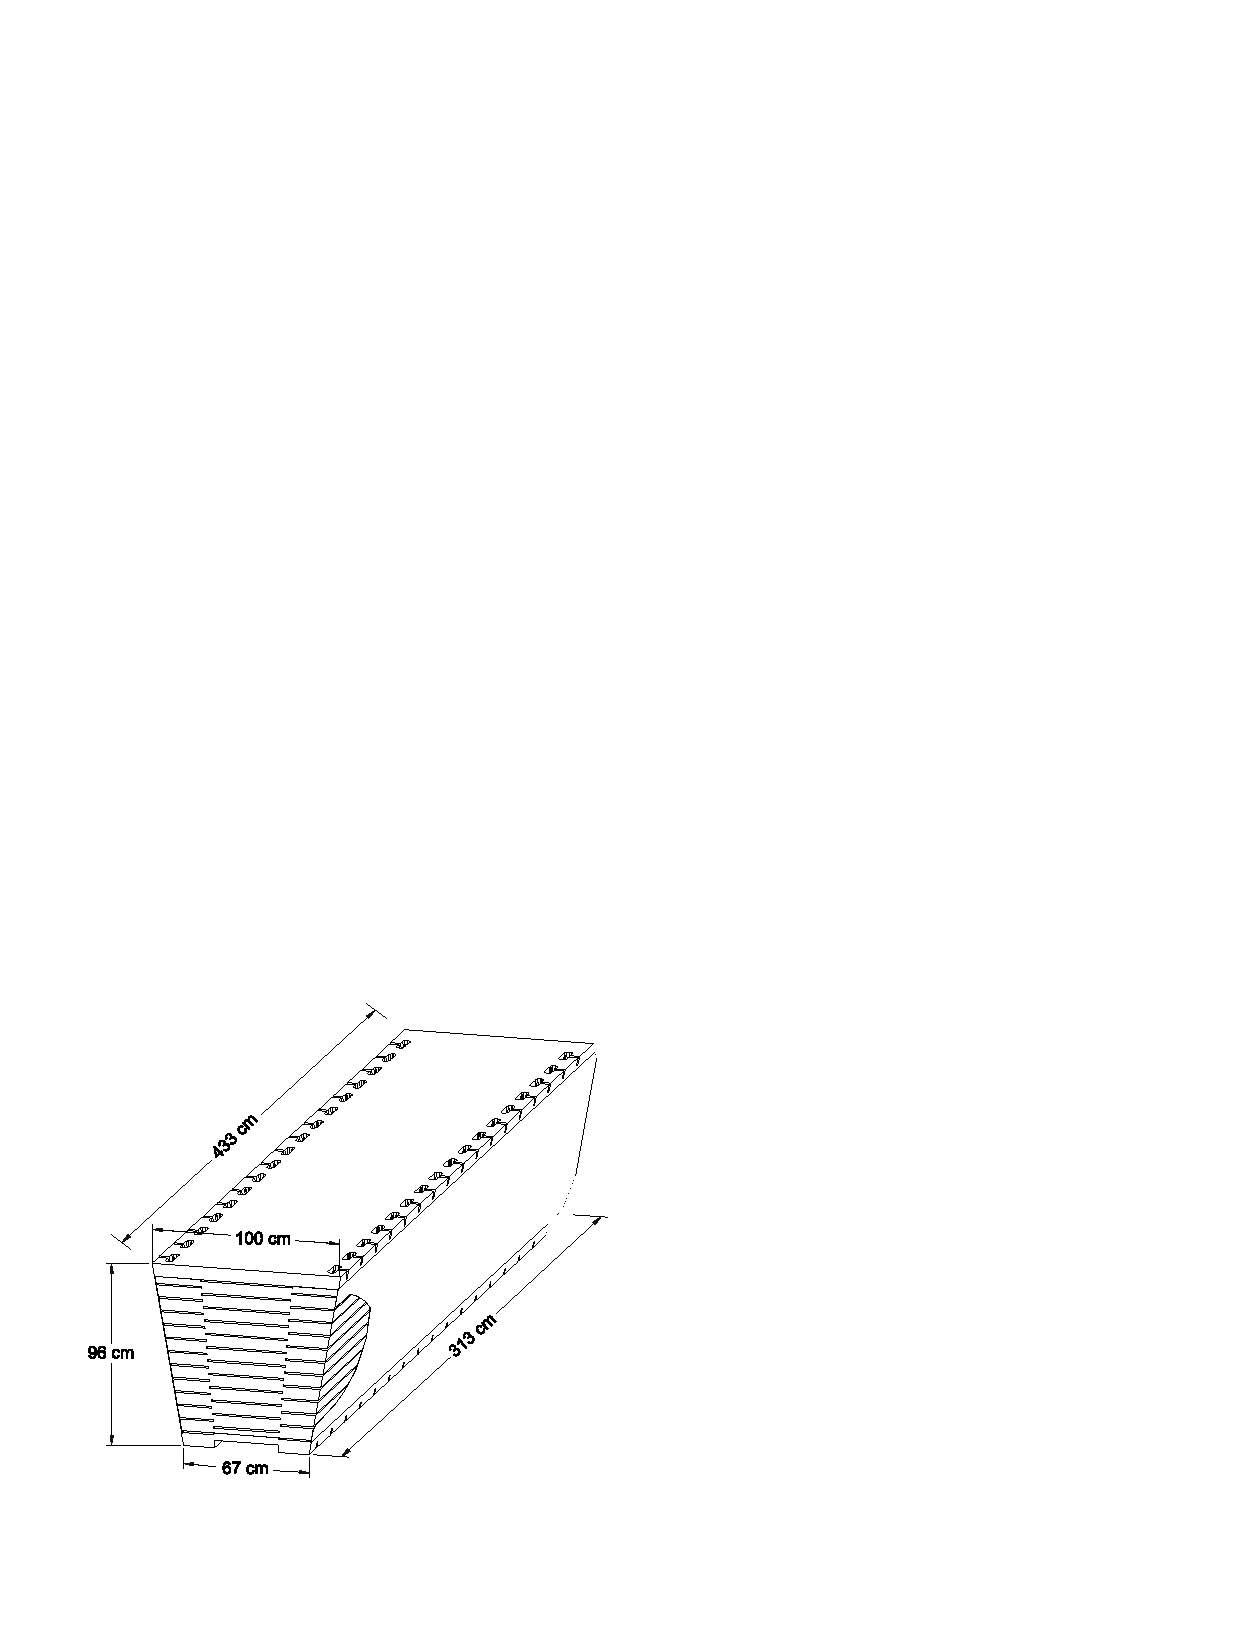
\includegraphics[width=.45\textwidth]{figures/hcal_wedge.pdf}
      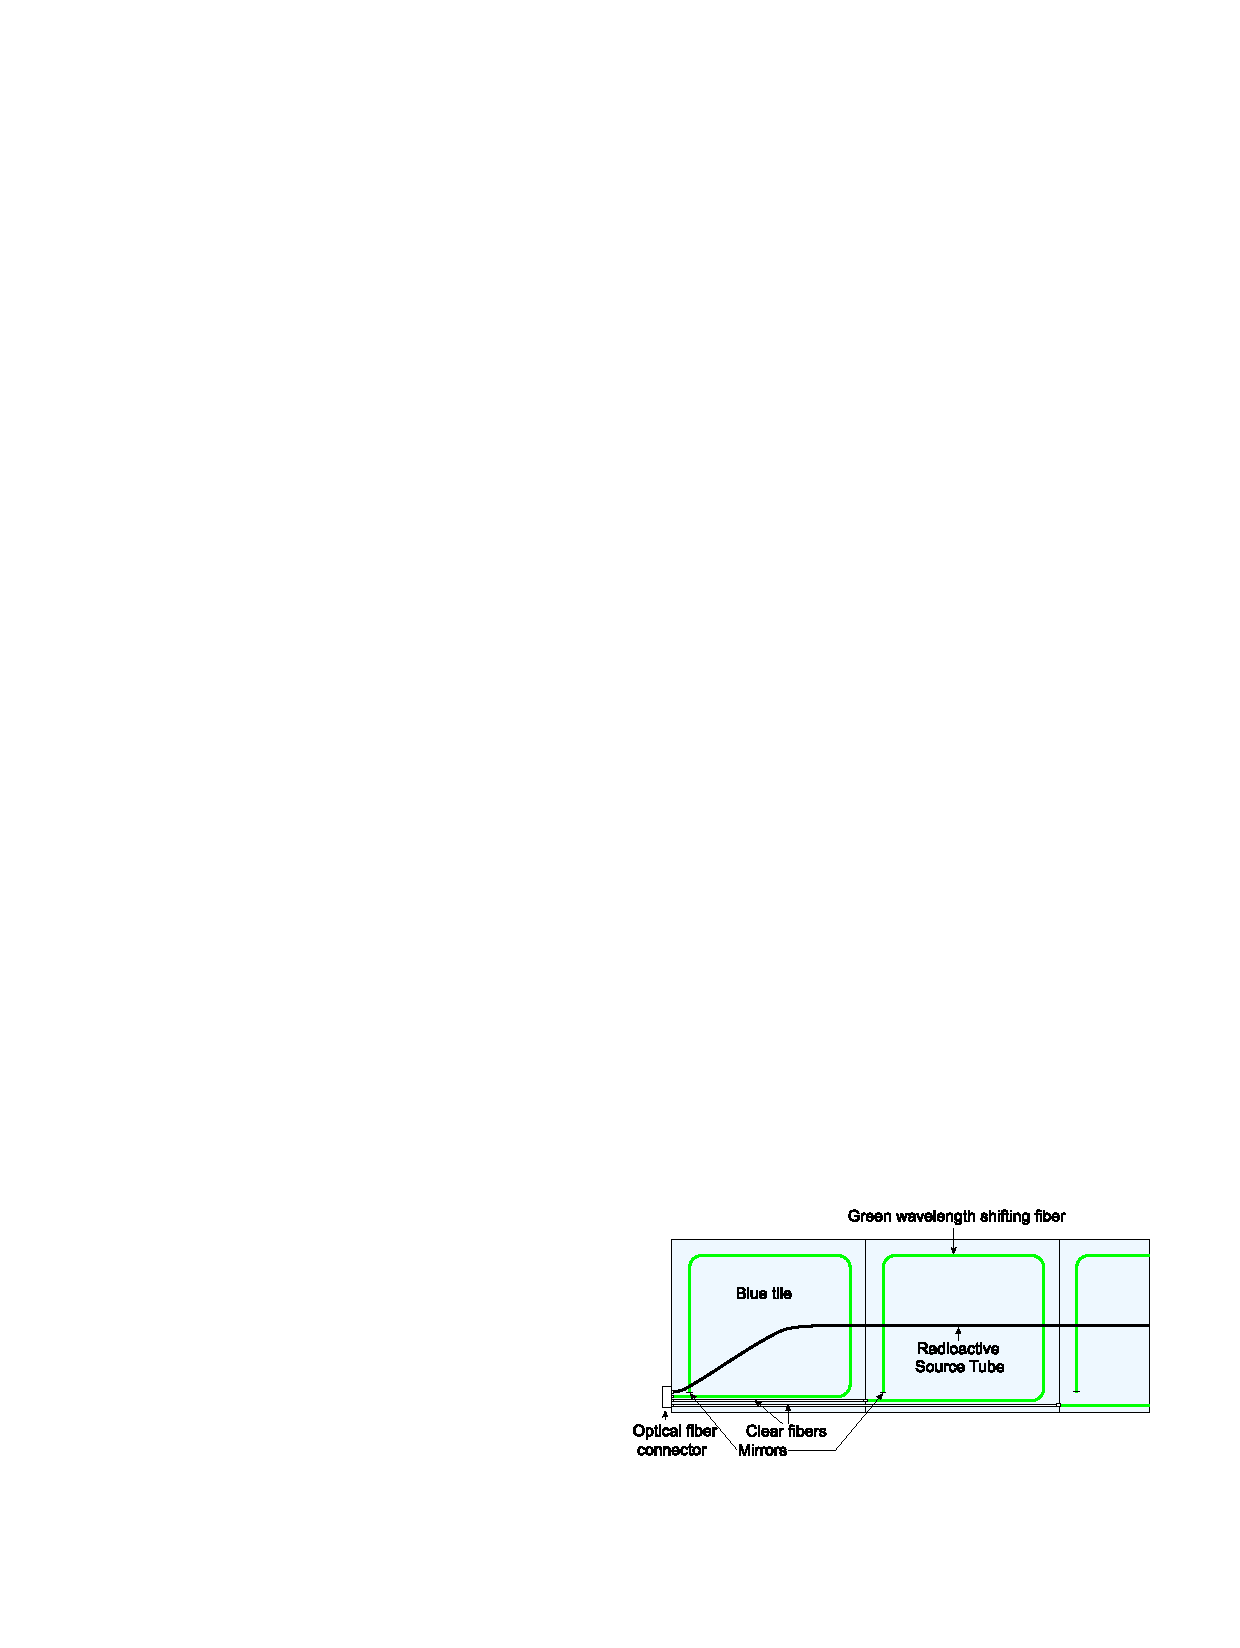
\includegraphics[width=.45\textwidth]{figures/hcal_scintillator.pdf}
      \caption{Shown on the left, a wedge of the HCAL in the barrel. The interior of the wedge is brass, and the shown slots have the scintillator modules (shown to the right) inserted so that secondary particles made in interactions with the brass will pass through them and have their energy measured. To the right, a scintillator module is shown, when a charged particle passes through the scintillator, light is generated and collected by the wavelength shifting fiber shown in green. When scintillation light is collected by the fiber, it releases green light that travels down to the clear fiber via total internal reflection and sent to be collected by photo sensors. Taken from \cite{cms_hcal_wedge}.}
      \label{fig:hcal_wedge}
    \end{figure}

    Figure \ref{fig:hcal_wedge} shows the general design of an HCAL wedge in the barrel region. Layers of brass are interspersed with scintillator strips that read out the energy of secondary particles created in the hadronic interaction. In terms of nuclear interaction lengths, the HCAL goes from about 5 nuclear interaction lengths at $\eta = 0$ up to about 10 at $\eta \ge 1.3$. Due to the shallow depth in the barrel, an outer layer of scintillator is added outside the magnet, essentially using the magnet as an absorber layer. This outer layer is called the HO and runs in the range $\eta \in [0, 1.3]$. Figure \ref{fig:hcal_layout} shows a cross-section of the HCAL including the HB, HE, and HO. With the HO in place, the minimum number of interaction lengths across the HCAL is increased to almost 12 except in the transition region between the endcap and barrel.\cite[pg. 138]{cms_jinst}

    \begin{figure}[h!]
      \centering
      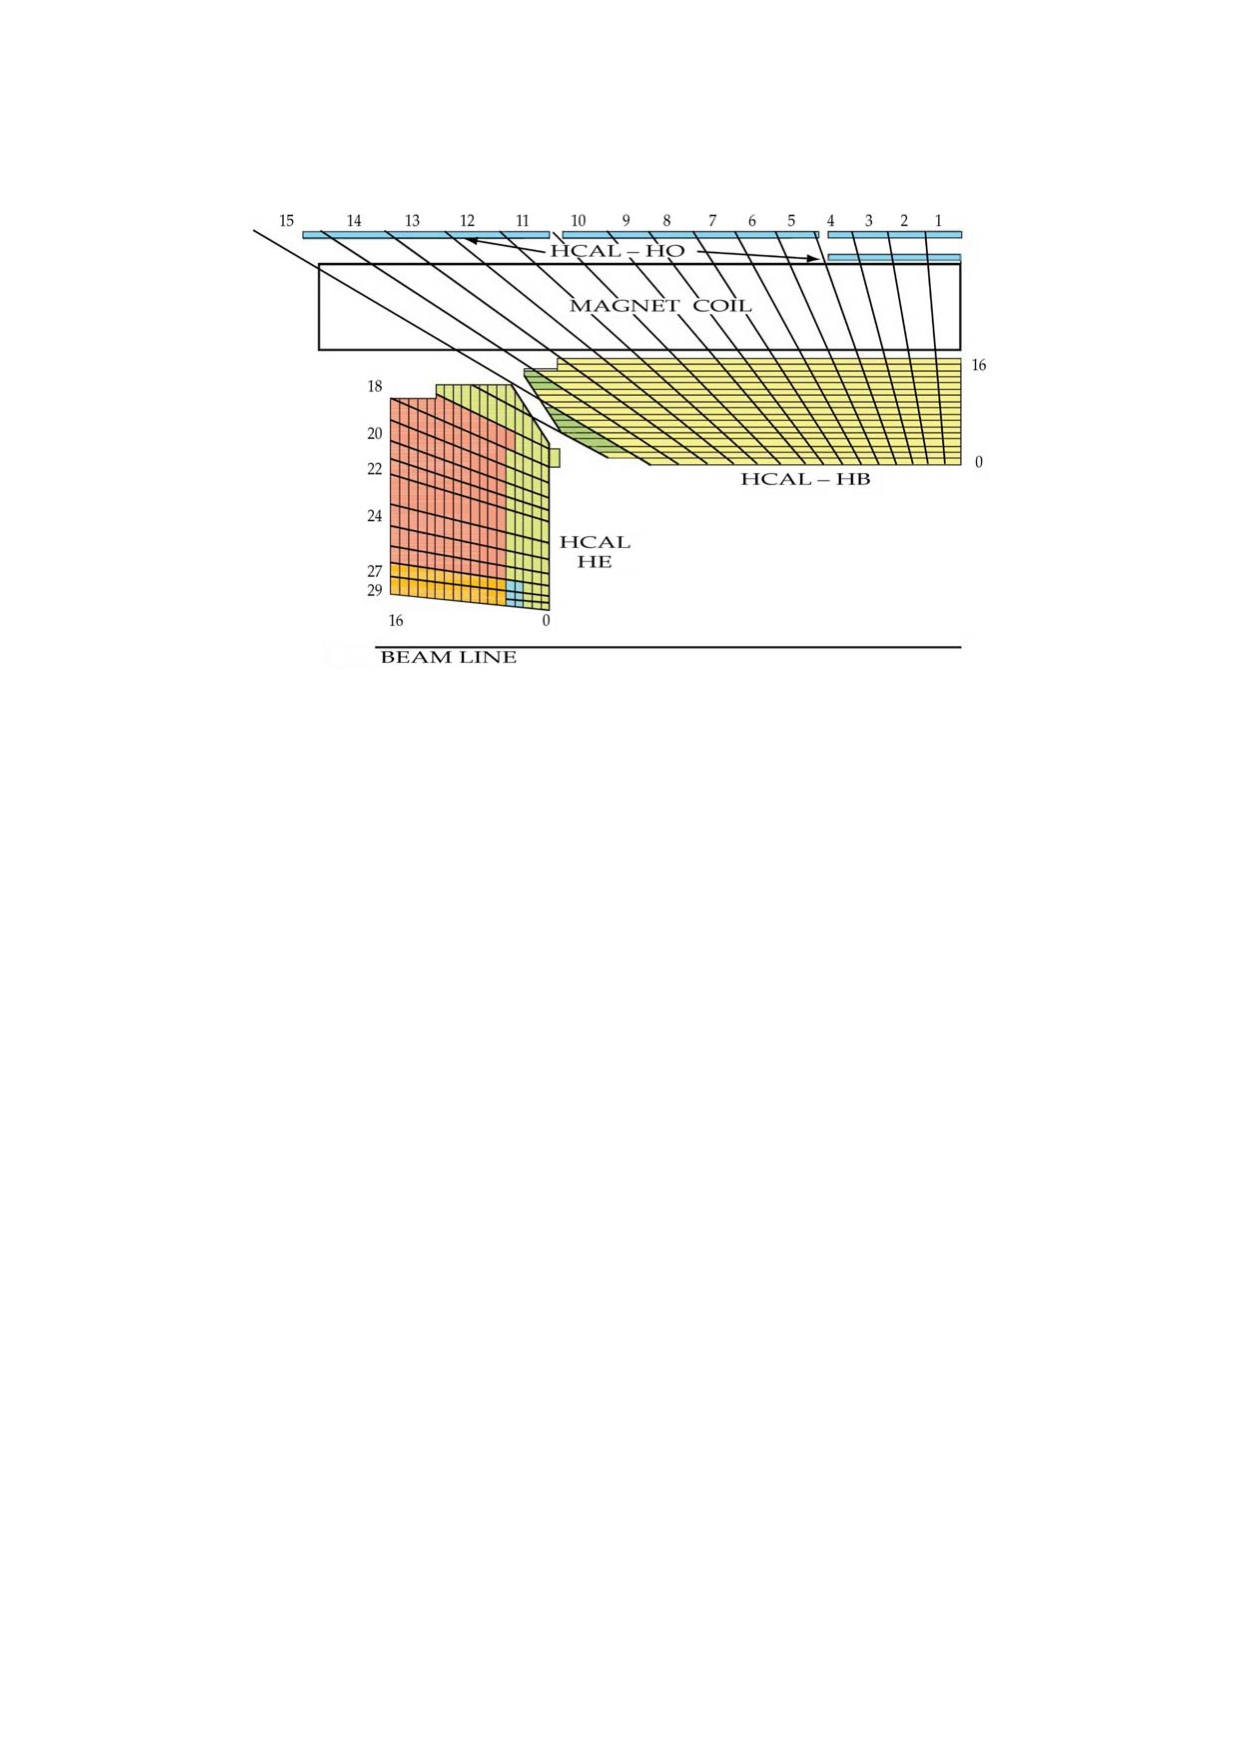
\includegraphics[width=.9\textwidth]{figures/cms_hcal_layout.pdf}
      \caption{The a cross-sectional view of the CMS hadronic calorimeter. Taken from \cite{cms_jinst}.}
      \label{fig:hcal_layout}
    \end{figure}

    Sampling calorimeters again work on the principle of scintillation, however, HCALs are meant to measure energy from neutral particles as well as charged hadrons. The strategy used in sampling calorimeters is to place dense material with many nuclei in front of the incident particles. Hadronic interactions are much more complicated than the photon and electron interactions in the ECAL because the initial state particles can vary, but in general the expected product of inelastic collisions are charged pions, which create electromagnetic cascades, and neutral particles like the $\eta$ and $\pi^0$ which quickly decay to photons. \cite[sec 35.9.2]{PDG} \cite{green_detectors} Neutron capture can also occur which makes photons that are typically out of the electronics detection capability.\todo{This is so confusing, how the hell can you say you get almost always pions for any hadronic particle?} The hadronic cascade of particles then leads into the scintillating material where scintillation light is generated and collected. Again, the amount of light collected is proportional to the energy of the charged particle \todo{why? also is the light from the $\eta$ and $\pi^0$ absorbable by the WSF?}.

    In the CMS HCAL, the absorber layers are made of brass, and the scintillator material is a proprietary plastic material, Kuraray SCSN81\footnote{excluding the very first layer where the absorber metal is stainless steel and the plastic scintillator is Bicron BC408. The very last layer also has stainless steel as the absorber metal.}. The HCAL is broken into three physical sections: the barrel (HB) extending to $\abs{\eta} \le 1.4$, the slightly overlapping endcap (HE) extending between $\abs{\eta} \in (1.3,3)$, and the slightly overlapping forward detector (HF) covering the range $\abs{\eta} \in (2.9,5)$. In this analysis, we do not use jets with energy measurements from the forward detector, that is we veto jets with $\eta > 3$.


  \subsection{The Muon System}
    The outer-most detection subsystem on CMS are the muon chamber. Muons literally put the ``M" in CMS, they are an extremely important particle for LHC physics for several reasons. \cite[sec 1.2]{muon_tdr}

    \begin{enumerate}
     \item Their production is associated with the electroweak sector, which includes the Higgs boson.
     \item They have a long enough lifetime that they can make it through the entire detector, making them easily identifiable and allowing for good momentum resolution due to their long track.
     \item Their radiative losses in the tracking system and ECAL are much smaller than electrons due to their heavier mass. They also don't deposit much energy in the HCAL because they don't interact via the strong force.
    \end{enumerate}

    The muon system on CMS is made up of three different types of detectors, all based on gas ionization.
    \begin{enumerate}
     \item{Drift Tubes} Tubes of 
     \item{Cathode Strip Chambers}
     \item{Resistive Plate Chambers}
    \end{enumerate}


    \begin{figure}[h!]
      \centering
      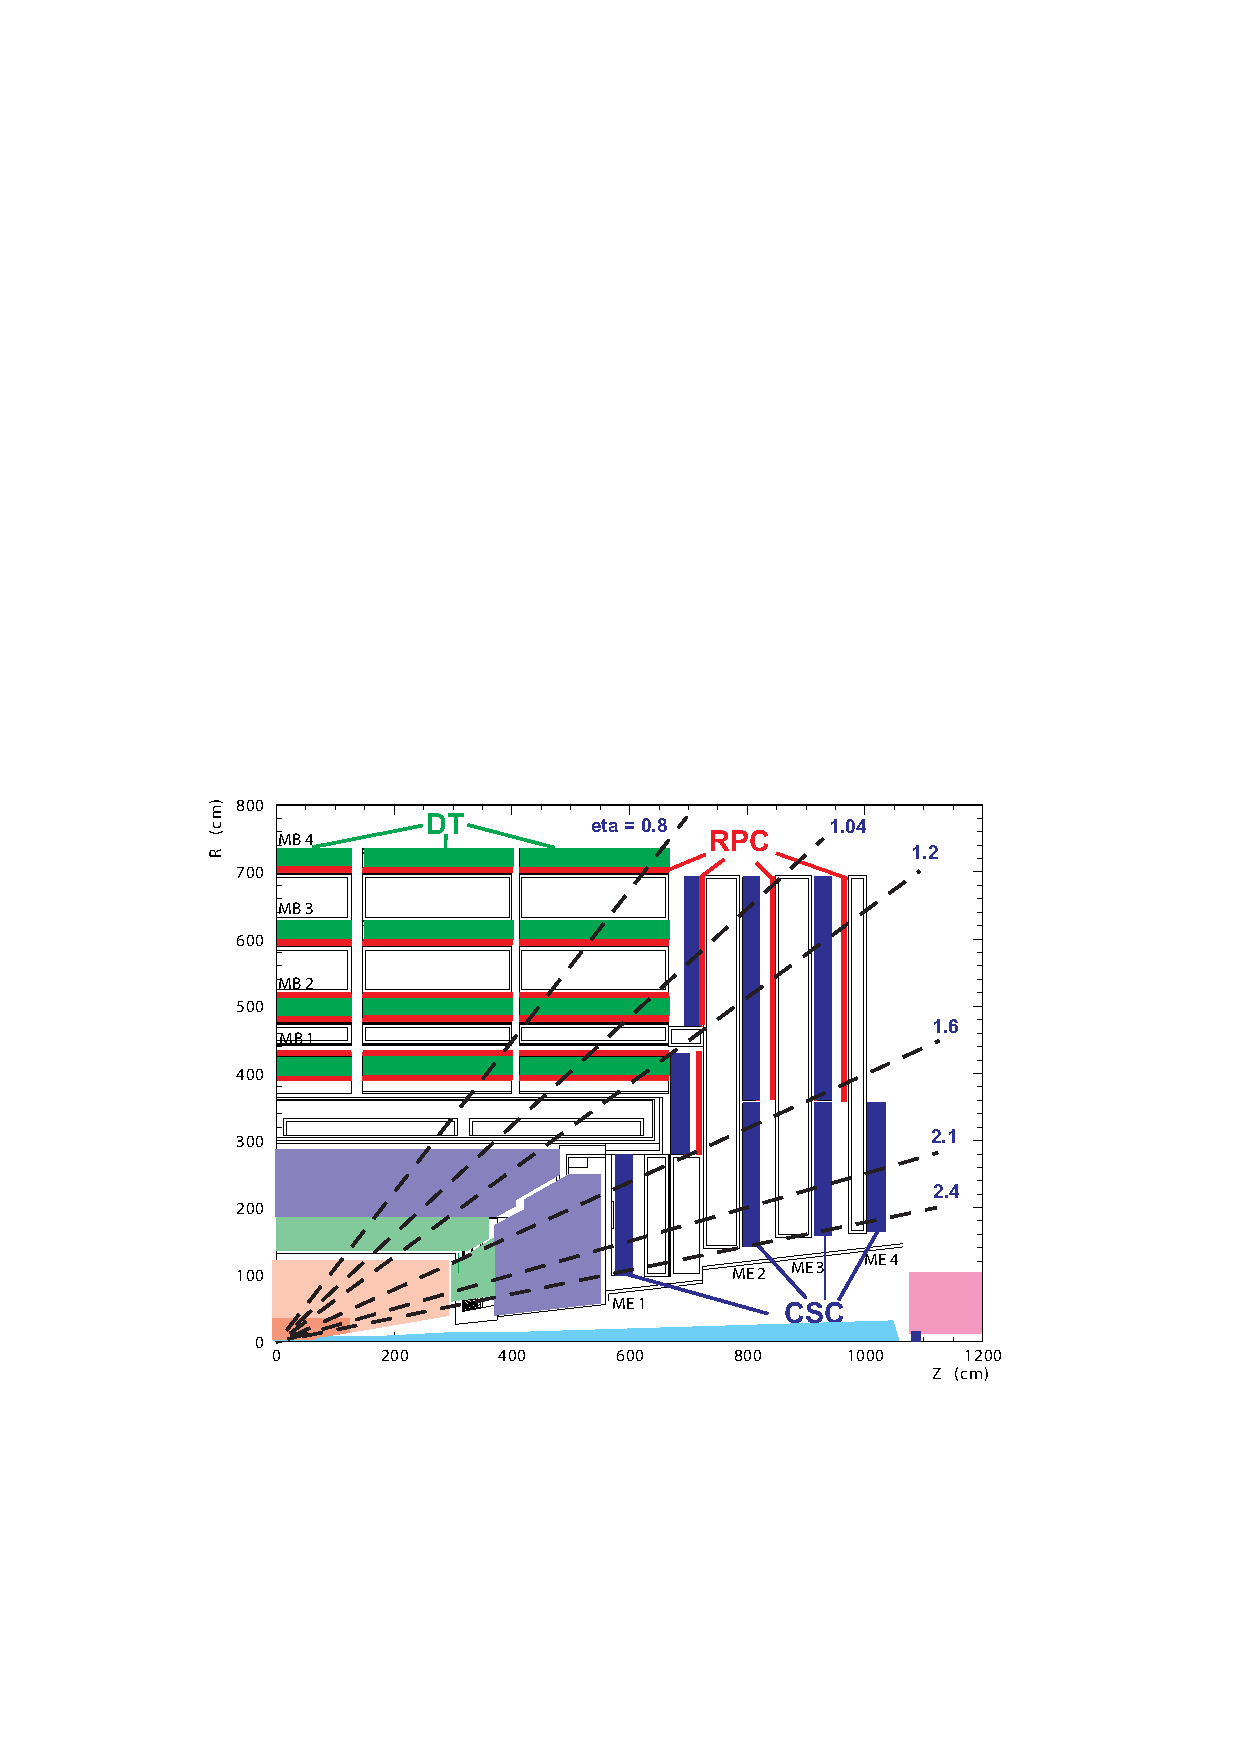
\includegraphics[width=.9\textwidth]{figures/muon_system.pdf}
      \caption{A cross-sectional view of the CMS muon system. In the barrel, with $\abs{\eta}<1.2$, drift tubes (DTs) and resistive plate chambers (RPCs) are used. In the end cap, $\abs{\eta} \in (1.2,2.4)$, RPCs and cathode strip chambers (CSCs) are used. Taken from \cite{cms_tdr}.}
      \label{fig:muon_system}
    \end{figure}

  \subsection{Fiducial Area} \label{sec:fiducial_area}
    the weird eta deadzone really effects electrons and we want symmetry between electrons and muon \ref{sec:inner_tracker}. very forward stuff, $\abs{\eta}<2.4$. 
  \subsection{Event Triggering} \label{sec:event_triggering}
    trigger turn ons, list the triggers we use, Level 1 and HLTs? Trigger efficiency 
\section{Physics Objects}
  \subsection{Particle flow and jet clustering} \label{sec:particle_flow}
    reconstruction efficiency
  \subsection{Vertex Selection} \label{sec:vertex_selection}
    \todo{Rewrite: We require the presence of at least one primary vertex satisfying the standard quality criteria; 176 namely,vertexisnotfake,ndf>4,ρ<2cm,and|z|<24cm.}
  \subsection{Electron Measurement Pipeline} \label{sec:electron_measurement_pipeline}
    Tracker, ecal, distinguishing between electrons and muons. Cite the CMS paper on electron energy reco.. \cite{Electron_reco}
  \subsection{Muon Measurement Pipeline} \label{sec:muon_measurement_pipeline}
    Tracker muons, global muons, muon system
  \subsection{Photon Measurement Pipeline}
    ECAL measurements, lepton conversions. Photons probably pair produce in higher eta ranges, how does that work?
  \subsection{Jets} \label{sec:jets}
    Describe charged hadron subtraction, JECs ~\cite{JERC}, \cite{JEC_2016}
    pfCHSjets with L1FastL2L3 corrections (MC), L1FastL2L3L2L3residual corrections (data).
    \verb=Summer16_23Sep2016V3= JEC payload used to correct jets
    Need to put in blurbs about L1 Pile Up Corrections, L2L3 MC-Truth Corrections, and L2L3Residual Corrections (data only). Short descriptions here: https://twiki.cern.ch/twiki/bin/view/CMS/IntroToJEC 

    pfjetID

    Good info in Vince's Thesis and here: https://arxiv.org/pdf/1607.03663.pdf
    Roughly: L1 -- (pileup offset correction) pileup correction use QCD MC to get avg energy change to jet with and without pileup overlay. Look in 2D plane of $\eta$ and \pt, get correction.
    L2L3 -- (simulated response correction) Look at dijet events in MC, see how energy reco is different across \pt and $\eta$, correct for it.
    L2L3 Residual -- (Residual Corrections for data) Make MET 0 in dijet/ZJet/GammaJet events.

    jet energy mismeasurements are a function of the absolute scale of energy
  \subsection{B-Tagging} \label{sec:b-tagging}

  \subsection{MET Reconstruction} \label{sec:MET_reco}
    Make sure to add bits about sources of MET and the Type 1 correction
  \subsection{MET Filters} \label{sec:met_filters} 
    We apply certain filters that kill events, these are called MET filters but include things like beam halo as well.

\section{Monte Carlo} \label{sec:monte_carlo}
  Physics generated using Madgraph 5 interfaced with pythia8 for showering. List samples and their generator.
  SUSY models are also simulated using the madgraph package, but are then passed through the fastsim toolkit \cite{fastsim} rather than the full GEANT simulation. Statistical uncertainty in MC.
  \subsection{Summary of Simulated Samples} \label{sec:summary_of_simulated_samples}
    
    In this section we list all the Monte Carlo (MC) samples used for this analysis as well their generator and detector simulation.

    In this section we list the MC samples used for the \pt reweighting closure test.
      \begin{table}[htb]
        \begin{center}
          \scriptsize
          \caption{\label{tab:closuremc} List of MC samples used for the closure test.}
          \begin{tabular}{l|l|c}  
            \hline
            \hline
            Process & Dataset Name                                                             & Cross Section [pb]\\
            \hline
            \gjets   & \verb=/GJets_DR-0p4_HT-40To100_TuneCUETP8M1_13TeV-*-v1=                & 18560    \\
                     & \verb=/GJets_DR-0p4_HT-100To200_TuneCUETP8M1_13TeV-*-v1=               &  5000    \\
                     & \verb=/GJets_DR-0p4_HT-200To400_TuneCUETP8M1_13TeV-*-v1=               &  1079    \\
                     & \verb=/GJets_DR-0p4_HT-400To600_TuneCUETP8M1_13TeV-*-v1=               &   125.9  \\
                     & \verb=/GJets_DR-0p4_HT-600ToInf_TuneCUETP8M1_13TeV-*-v1=               &    43.36 \\
            \hline   
            \zjets   & \verb=/DYJetsToLL_M-50_TuneCUETP8M1_13TeV-*_ext1-v2=                     &  6021    \\
                     & \verb=/DYJetsToLL_M-50_HT-100to200_TuneCUETP8M1_13TeV-*_ext1-v1= &   181.3   \\
                     & \verb=/DYJetsToLL_M-50_HT-200to400_TuneCUETP8M1_13TeV-*_ext1-v1= &    50.42  \\
                     & \verb=/DYJetsToLL_M-50_HT-400to600_TuneCUETP8M1_13TeV-*_ext1-v1= &     6.984 \\
                     & \verb=/DYJetsToLL_M-50_HT-600to800_TuneCUETP8M1_13TeV-*-v2= &     1.681 \\
                     & \verb=/DYJetsToLL_M-50_HT-800to1200_TuneCUETP8M1_13TeV-*-v1= &    0.7754  \\
                     & \verb=/DYJetsToLL_M-50_HT-1200to2500_TuneCUETP8M1_13TeV-*-v1= &   0.1862  \\
                     & \verb=/DYJetsToLL_M-50_HT-2500toInf_TuneCUETP8M1_13TeV-*-v1= &    0.004385  \\
            \hline
            Campaign & \verb=*madgraphMLM-pythia8/RunIISummer16MiniAODv2=                       & \\
                     & \verb=-PUMoriond17_80X_mcRun2_asymptotic_2016_TrancheIV_v6*/MINIAODSIM= & \\

            \hline
            \hline
          \end{tabular}
          \end{center}
      \end{table}

\section{Datasets} \label{sec:datasets}
We use dilepton trigger events, as will be described in section \ref{sec:leptonic_final_states}